% When Is Surrogate-Assisted Multiobjective Ensemble Weighting Trustworthy?
% Manuscript source in Elsevier's elsarticle class (single column, author-year references).
% Build with:  tectonic main.tex             (identified manuscript)
%              tectonic main_anonymized.tex  (copy for double-anonymized review; author details on title_page.tex)
% Figures are produced by build_assets.py from the frozen R=30 artifacts (tag pco213-postwork-r30).
\providecommand{\ifanon}[2]{#2}% #1: text of the anonymized review copy; #2: text of the identified manuscript
\documentclass[preprint,11pt,authoryear]{elsarticle}

\usepackage[T1]{fontenc}
\usepackage[utf8]{inputenc}
\usepackage[english]{babel}
\usepackage{lmodern}
\usepackage[a4paper,margin=2.5cm]{geometry}
\usepackage{amsmath,amssymb}
\usepackage{booktabs}
\usepackage{graphicx}
\usepackage{longtable}
\usepackage{multirow}
\usepackage{siunitx}
\usepackage[hidelinks]{hyperref}
\usepackage[capitalise,noabbrev]{cleveref}
\usepackage{microtype}
\usepackage{xcolor}
\usepackage{caption}

% absorb the last few points of overfull in justified paragraphs
\setlength{\emergencystretch}{1.5em}
\captionsetup{font=small,labelfont=bf}
\graphicspath{{figures/}}
\bibliographystyle{elsarticle-harv}
\journal{Engineering Applications of Artificial Intelligence}
% first-page footer without the compile date (the class default overruns the text width with this journal name)
\makeatletter
\def\ps@pprintTitle{\let\@oddhead\@empty\let\@evenhead\@empty
  \def\@oddfoot{\footnotesize\itshape Preprint submitted to \@journal\hfill}\let\@evenfoot\@oddfoot}
\makeatother

\newcommand{\wvec}{\mathbf{w}}
\newcommand{\simplex}{\Delta^{M-1}}
\newcommand{\igdp}{\mathrm{IGD}^{+}}
\newcommand{\hv}{\mathrm{HV}}
\newcommand{\rext}{R^{2}_{\mathrm{ext}}}

\begin{document}

\begin{frontmatter}
\title{When Is Surrogate-Assisted Multiobjective Ensemble Weighting Trustworthy? A Replicated Study of Mixture
Designs, Scheff\'e Surfaces and Normal Boundary Intersection on the Classifier-Weight Simplex\tnoteref{abbrev}}
\tnotetext[abbrev]{Abbreviations: CHIM, convex hull of individual minima; DoE, design of experiments; NBI, Normal
Boundary Intersection; NSGA-II, non-dominated sorting genetic algorithm II; ROC-AUC, area under the receiver operating
characteristic curve; RSM, response surface methodology.}
\ifanon{}{%
\author[a,b]{Caio Tertuliano Ribeiro\corref{cor1}}
\ead{caio.tertu@hotmail.com}
\author[b]{Matheus Costa Pereira}
\author[b]{Anderson Paulo de Paiva}
\cortext[cor1]{Corresponding author.}
\affiliation[a]{organization={Manufacturing Optimization and Innovation Technology Center (NOMATI)},
  city={Itajub\'a}, state={MG}, country={Brazil}}
\affiliation[b]{organization={Institute of Industrial Engineering and Management (IEPG), Universidade Federal de
  Itajub\'a}, addressline={Av.\ BPS 1303}, postcode={37500-903}, city={Itajub\'a}, state={MG}, country={Brazil}}
}

\begin{abstract}
Choosing soft-voting ensemble weights is a mixture experiment addressed by an established mixture-design,
response-surface and Normal Boundary Intersection pipeline. The artificial-intelligence contribution is a diagnosis
of when that pipeline can be trusted, not a new method; the engineering application is designing weighted classifier
ensembles under a measured deployment cost. Three arms differing in objective and anchor sources ran on 30
overlapping, paired partitions of four public financial-services datasets, with controls the framework lacks: a
reliability gate fixed beforehand, out-of-fold real-objective revalidation, a reference core without the methods' search output,
and an untouched confirmation holdout. Gate passes ranged from 0/30 to 30/30. Under the optimized continuous cost, real anchors beat surrogate ones on both primary endpoints in
every partition of the two datasets whose surfaces for the area under the receiver operating characteristic curve
almost never passed, and in 23--24 of 30 elsewhere (significant after an assumed-dependence correction only on Santander). On those two, anchor misplacement was the largest observed failure; a control traced most of it to injected extreme
solutions. The gate detected unusable surfaces but not misplaced anchors. Continuous and step deployment costs
disagreed on the winning candidate set in 8--24 of 30 partitions and the anchor effect's direction on one dataset,
a post hoc check finding the step-cost reference less converged.
The non-dominated sorting genetic algorithm II (NSGA-II), given about twice the metamodel-free arm's weight-vector
evaluations and returning larger sets, outperformed it. The diagnosis concerns one-shot pipelines without infill; four datasets establish a
pattern, not a general rule.

\end{abstract}

\begin{keyword}
ensemble weighting \sep mixture design of experiments \sep response surface methodology \sep normal boundary
intersection \sep surrogate-assisted multiobjective optimization \sep inference cost
\end{keyword}
\end{frontmatter}

\section{Introduction}
\label{sec:intro}

A weighted average of several classifiers' predicted probabilities is among the oldest and most reliable devices in
applied machine learning \citep{hansen1990neural,wolpert1992stacked,kittler1998combining,caruana2004ensemble}. Its
weights are not free parameters: to keep the output a probability they must be non-negative and sum to one, and
non-negativity with normalization is what makes stacked combinations stable \citep{breiman1996stacked}. The feasible
set is the unit simplex, so ensemble weighting is a \emph{compositional} optimization problem.

That has a methodological consequence: optimization over a simplex is the subject of mixture experiments, a mature
branch of experimental design \citep{scheffe1958mixtures,scheffe1963simplexcentroid,cornell2002mixtures}. The
classifiers are the components, a pure vertex is a single model, the centroid uniform soft voting, and a Scheffé
polynomial the natural response surface. The correspondence is exact and already exploited for portfolio weights
\citep{mendes2016portfolio_mde,leal2022portfolio_doptimal_mde} and neural-network ensembles
\citep{moreira2021ann_ensemble_mde}, and combined with Normal Boundary Intersection for forecast combination
\citep{bacci2019nbi_mixture}, load forecasting \citep{rocha2025ensemblestlf} and multiobjective engineering
optimization \citep{pereira2025hybrid}. Most directly, \citet{kwon2024ensemble} treat five heterogeneous
\emph{classifiers}' weights as mixture components and maximize a Scheffé polynomial of accuracy or $F_1$ on eleven
tabular binary datasets.

\textbf{We therefore claim no part of that construction:} mixture design over combination weights, a Scheffé surrogate
over the simplex, and NBI on that surrogate are established prior work, individually and for classifier ensembles.
What is not established is whether the construction stays \emph{trustworthy} once the problem becomes genuinely
multiobjective. That is the question this paper addresses.

\subsection{Why the transfer is not routine}

The applications in which this framework matured share three properties that classifier ensembles do not.

First, \emph{the responses are smooth}: tool life or process cost varies smoothly with cutting speed, where a
low-order polynomial is a defensible local model. The area under the receiver operating characteristic curve (ROC-AUC)
is instead a rank statistic, piecewise constant in the weights. A richer design alone cannot remove the approximation
bias of an unsuitable model class, so whether a low-order polynomial represents such a response adequately has to be
measured on unseen compositions rather than assumed.

Second, \emph{the decision variables are the mixture}. When the simplex holds scalarization weights, as in the lineage
above, NBI's anchors are optima of the surrogate in another space; when it holds the decision variables themselves,
the anchors are feasible-region points (often vertices), so an anchor error displaces the geometry in which every
subproblem is posed. NBI derives its whole search geometry from the payoff matrix of individual optima
\citep{das1998nbi}, so errors there propagate globally. That misplaced anchors damage the construction is established:
the worst criterion values read off a payoff table can differ substantially from the true worst values over the
efficient set \citep{isermann1988payoff}, the nadir point is hard to estimate \citep{deb2010nadir}, and the choice of the individual
minima has itself been treated as a design lever \citep{herrmann2026nonextreme}. What that literature, and the
normalization remedies built on it \citep{messac2003normalized}, asks about is estimating the \emph{true} objectives;
none of it is about a surrogate standing in for them.

Third, \emph{one objective is a step function}: a model with any non-negligible weight must be loaded and executed,
one with none costs nothing, so deployment cost is not proportional to a weight. A method requiring differentiable
objectives can only optimize a continuous relaxation, with no guarantee that it and the quantity actually paid agree
about which solution is best.

Each can break a different part of the pipeline (the model class, the search geometry, the objective definition),
and none is visible in the aggregate fit statistics such studies conventionally report.

\subsection{Approach}

We decompose the framework. Because the ensemble output is linear in the weights and base-model probabilities can be
cached, evaluating a weight vector on the true objectives costs one matrix--vector product ($0.4$ to
$2.1$~milliseconds here) --- cheap enough to run the \emph{same} NBI three times per replication, changing only where
objectives and anchors come from.

\begin{itemize}
\item \textbf{NBI-A} optimizes the Scheffé surfaces with anchors from their own optima: the inherited construction and
our control.
\item \textbf{NBI-B} optimizes the same surfaces with anchors from the real single-objective optima; A versus B
isolates \emph{anchor misplacement}.
\item \textbf{NBI-C} drops the metamodel and runs the same NBI on the exact out-of-fold objectives --- a
metamodel-free NBI in the published sense of \citet{gellerich2023doenbi}, whose subproblems are physical experiments;
B versus C isolates residual \emph{interior surrogate error}.
\end{itemize}

All three arms fit their surfaces once from a fixed design and then optimize. This is the \emph{sequential} form of
surrogate-assisted optimization \citep{tabatabaei2015survey} --- one-shot, with no infill --- and it is the form the
lineage above uses; nothing here tests model-managed, infill-based surrogate-assisted optimizers such as ParEGO,
MOEA/D-EGO or SMS-EGO \citep{knowles2006parego,zhang2010moeadego,ponweiser2008smsego}, which evaluate new points on
the true objectives inside the search loop and exist precisely to repair the kind of surrogate error diagnosed here.
Every conclusion in this paper is scoped to the one-shot, no-infill case (\cref{sec:rel:surrogate}).

We also run NSGA-II on the same objectives, with about twice as many weight-vector evaluations as NBI-C. Four controls
the lineage does not contain surround the decomposition: external validation of every surface on 100 unseen
compositions, with a reliability gate fixed before the replicated benchmark; revalidation of every candidate on the
true objectives before any indicator; an empirical Pareto reference whose sampled core of at least $10^{5}$ points per
replication contains no output of the compared methods and is checked for convergence, then augmented with every
candidate set for scoring; and an untouched holdout never used for fitting, weighting, thresholding or selection.

Four public binary tabular datasets --- customer-transaction prediction (Santander), insurance-claim processing (BNP
Paribas Cardif), auto-insurance claim prediction (Porto Seguro) and consumer-credit default (UCI credit) --- are
partitioned 30 times each, giving 120 replications with recorded seeds. The four prediction tasks differ, but all four
come from financial-services applications, so any cross-dataset statement is made within a single application domain.
Because partitions of one dataset overlap heavily, we treat the replication distribution as partition sensitivity, not
a sample from a population: comparisons are paired by partition and tested with the Nadeau--Bengio correction
\citep{nadeau2003inference}, which the descriptive bootstrap and Wilson intervals do not carry; the dataset is the
unit of generalization; and nothing is pooled across the 120 replications.

\subsection{Research questions}

\begin{enumerate}
\item[\textbf{RQ1}] How accurately do Scheffé surfaces predict ensemble performance on compositions they have not
seen, and does this depend on the dataset, on the metric, or on both?
\item[\textbf{RQ2}] How stable are the fitted surfaces across resampling, and does the classical mixture-design
reading of the interaction coefficients survive confrontation with the real objectives?
\item[\textbf{RQ3}] What goes wrong when NBI is anchored on surrogate optima?
\item[\textbf{RQ4}] Does replacing surrogate anchors with real ones repair the front, and does the reliability gate
predict when this is necessary?
\item[\textbf{RQ5}] How does surrogate-assisted NBI compare with metamodel-free NBI, what does the difference cost,
and how do both compare with a canonical evolutionary optimizer on the same objectives?
\item[\textbf{RQ6}] How large is the actual conflict between discrimination and calibration?
\item[\textbf{RQ7}] Does the definition of deployment cost change which method wins?
\item[\textbf{RQ8}] Do solutions selected on out-of-fold data transfer to an untouched holdout?
\item[\textbf{RQ9}] Would the first ten replications have produced the same conclusions?
\end{enumerate}

\subsection{Contributions}

\begin{enumerate}
\item \textbf{A controlled decomposition of a one-shot surrogate-assisted multiobjective pipeline into surrogate
error, anchor misplacement and solver behaviour}, through three NBI variants defined by two methodological factors.
The ingredients are not new and are not claimed: anchor and ideal/nadir misestimation is an established failure mode
\citep{isermann1988payoff,deb2010nadir,he2021normalization}, the choice of individual minima has already been treated
as a design lever \citep{herrmann2026nonextreme}, and NBI run metamodel-free on measured objectives with real anchors
is published \citep{gellerich2023doenbi}. To the best of our literature search, no prior study computes the anchors
of a method built on the convex hull of individual minima (CHIM) both from a fitted surrogate and from the true
objectives on the same problem and compares the resulting fronts, so
what is new here is the surrogate \emph{provenance} of the anchor error and the controlled comparison of the two
constructions; the nearest ensemble-weighting precedent \citep{kwon2024ensemble} optimizes one metric at a time and
has no anchors or front.

\item \textbf{Evidence that, on two of the four datasets, anchor misplacement has the largest observed effect among
failures attributable to the surrogate pipeline.} Under the continuous cost the arms optimize, real anchors improve both
primary endpoints in 30 of 30 partitions on the two datasets whose ROC-AUC surfaces almost never pass the gate
(Santander and BNP Paribas), in 23 (IGD$^+$) and 24 (hypervolume) of 30 on Porto Seguro, and in 24 of 30 on UCI
credit; after correction the improvement is significant only on Santander. Removing the surrogate entirely, once
anchors are correct, adds much less on Santander and BNP Paribas, about as much on Porto Seguro, and three times as
much on UCI credit, where subproblem convergence rather than surrogate error dominates; the tie and the reversal
prevent a universal claim.

\item \textbf{A demonstration that an external reliability gate detects unusable surfaces but not misplaced anchors.}
On one dataset the two properties diverge: the partitions where surrogate-anchored NBI collapses are precisely those
where the parsimony rule selects a ROC-AUC surface that fits held-out compositions \emph{better} and passes the gate more
often. Surface quality and argmax quality are different properties, and only the second governs NBI.

\item \textbf{A replicated evaluation architecture for ensemble-weight optimization}: external surrogate validation,
real-objective revalidation, a reference whose sampled core contains no output of the compared methods, and holdout
confirmation, over 4 datasets $\times$ 30 partitions with paired inference and Nadeau--Bengio-corrected primary tests.
Three findings it overturned, one of them an artifact noted but not resolved in the ten-partition analysis, are
reported explicitly.

\item \textbf{Two findings about how these surfaces should be read.} The classical synergism criterion $\beta_{ij} >
|\beta_i - \beta_j|$ holds for the leading pair's fitted surfaces on all four datasets in every partition, yet the
real 50/50 blend beats its better member on only one. And the continuous cost these methods optimize disagrees with
the step cost deployment pays often enough to change the winning method in up to 24 of 30 partitions. That a change
of cost accounting can reorder
a comparison is known across ensemble and cascade architectures \citep{wang2022committees}; what is reported here is
the disagreement between two accountings applied to one and the same weight vector.
\end{enumerate}

We claim neither that NBI outperforms other multiobjective optimizers (NSGA-II, given about twice the weight-vector
evaluations of NBI's metamodel-free arm, outperforms that arm on all four datasets), nor that it produces more
uniformly spaced fronts, nor that any method here is a general-purpose recommendation. The contribution is the set of
conditions under which an established framework can and cannot be trusted in a new problem class, and the controls
needed to tell the difference. Both are stated for the one-shot, no-infill form of that framework, since no arm here
performs iterative infill.

\section{Related work}
\label{sec:related}

This section keeps only what bears on a novelty claim.

\subsection{Classifier ensemble weighting}
\label{sec:rel:weighting}

Weighted voting and weighted probability averaging are long established
\citep{hansen1990neural,kittler1998combining,dietterich2000ensemble,kuncheva2014combining}; the weights come from
stacked generalization
\citep{wolpert1992stacked,breiman1996stacked,leblanc1996combining,vanderlaan2007super,ledell2016auc}, greedy forward
selection \citep{caruana2004ensemble}, numerical optimization
\citep{zhang2011sparse,yao2018stacking,shahhosseini2022optimizing,hassan2026weighted,xu2026pseo} or theory
\citep{fumera2005theoretical}. Throughout, the simplex is almost always respected as a constraint rather than designed
over as an experimental region, and essentially all of this work is single-objective.

\subsection{Multiobjective ensemble optimization}
\label{sec:rel:moo}

Multiobjective ensemble learning divides by decision variable: the \emph{members}
\citep{abbass2003pareto,chandra2006ensemble,jin2008pareto}; a \emph{subset}
\citep{dossantos2008dynamic,qian2015pareto}; or --- the family relevant here --- \emph{continuous combination
weights} under conflicting criteria, optimized by metaheuristics
\citep{ekbal2011multiobjective,ekbal2013combining,bandyopadhyay2008amosa,onan2016multiobjective,rezaei2019multi,zhao2018multiobjective,vrugt2006multi,galvan2026simultaneous}
and surveyed in \citet{ribeiro2020ensemble}.

This family is therefore \emph{not} new, and we do not claim it. Absent from this cluster is any designed experiment
and fitted response surface over the weight simplex, any classical scalarization method such as NBI, and --- with the
partial exception of the sparsity term in \citet{zhao2018multiobjective} --- any treatment of deployment cost as an
objective. Fronts are rarely replicated over resampled partitions with corrected inference
\citep{demsar2006statistical}.

\subsection{Mixture experiments and response surfaces}
\label{sec:rel:mixture}

Mixture experiments address exactly the constraint set of \cref{eq:simplex}, through simplex-lattice designs and
Scheffé's canonical polynomials
\citep{scheffe1958mixtures,scheffe1963simplexcentroid,cornell2002mixtures,myers2016rsm}; because $\sum_i w_i = 1$,
their coefficients are not component effects in the ordinary sense \citep{piepel1982component}.

The classical reading of a positive interaction coefficient is \emph{synergistic blending}
\citep{cornell2002mixtures}: a statement relative to the chord, not relative to the better pure component, and the
distinction turns out to matter (\cref{sec:results:coefficients}).

Mixture designs are beginning to appear in machine learning
\citep{karl2023svem,leal2025mixtureweights,xie2023doremi,ye2025mixinglaws,liu2025regmix,chen2025aioli,thudi2025mixmin},
but share our formalism and not our object: none models the performance of a weighted \emph{prediction} ensemble.

The exception, and the closest prior art to this study, is \citet{kwon2024ensemble}: the weights of five heterogeneous
classifiers as mixture components, a Scheffé canonical polynomial of accuracy or $F_1$ fitted over a mixture design,
reduced by backward elimination and maximized subject to $\sum_i w_i = 1$, on eleven tabular binary datasets. The
simplex formulation, the mixture design over classifier weights and the Scheffé surrogate are therefore established
prior art for classifiers, and we claim none of them. What that study does not do is what this paper is about: it
optimizes one scalar metric at a time, so it has no Pareto front, no anchors and no NBI; it validates the fitted
polynomial only in-sample, against no separately sampled reference front; and it carries no cost objective.

\subsection{The DoE--RSM--NBI framework and its application to ensemble weights}
\label{sec:rel:lineage}

Normal Boundary Intersection \citep{das1998nbi} was introduced to obtain a distributed representation of the Pareto
boundary, by solving for each convex weight vector a subproblem that advances from the convex hull of individual
minima along a quasi-normal direction. It
is widely combined with response-surface metamodels in engineering optimization, and a substantial body of work applies
NBI to polynomial surfaces fitted from designed experiments
\citep{brito2014nbimse,costa2016nbimmse,lopes2016rpdmnbi,naves2017nbirfs,belinato2019mnbipca,almeida2022taguchinbi}.

Within that tradition, mixture designs have been used to schedule the NBI weights and to model post-Pareto criteria
over the weight simplex. \citet{mendes2016portfolio_mde} and \citet{leal2022portfolio_doptimal_mde} model portfolio
proportions with mixture designs; \citet{bacci2019nbi_mixture} builds a simplex lattice over time-series
forecast-combination weights, fits Scheffé models to factor scores of residual accuracy metrics and applies NBI to
those models; \citet{paula2019gatuning} crosses a mixture design over objective weights with genetic-algorithm
hyperparameters. \citet{pereira2025hybrid}\ifanon{}{, of which the present first author is a co-author,} extends the framework
with a mixture-design post-Pareto stage in which Scheffé polynomials of a generalized distance and of the entropy of
the weights are themselves optimized by a second NBI. Its anchors, like those of the rest of this literature, are the
individual optima of the surrogate surfaces --- the configuration we label NBI-A. \ifanon{A master's}{The first author's master's}
dissertation \citep{ribeiro2026dissertation} applies the same framework to hyperparameter optimization.

Most directly, \citet{moreira2021ann_ensemble_mde} determine neural-network ensemble weights by a mixture design, and
\citet{rocha2025ensemblestlf} combine a $\{3,5\}$ simplex-lattice design over the mixing weights of three neural
networks, a factor-analytic surrogate of correlated error metrics, NBI over those surrogates, and an entropy-based
post-Pareto choice, for short-term load forecasting. That is the present pipeline applied to a regression ensemble, and
its stated first contribution is casting ensemble-weight definition as a structured mixture-design problem.

\textbf{We therefore claim no part of this construction as new.} Our contribution begins where this literature stops:
none of these studies validates its mixture surrogate on unseen compositions, computes anchors from anything other than
the surrogate, revalidates its Pareto candidates on the true objectives, scores them against a separately sampled
reference, or replicates over resampled partitions.

\subsection{Surrogate-assisted multiobjective optimization}
\label{sec:rel:surrogate}

The broader surrogate-assisted literature \citep{jin2011surrogate,tabatabaei2015survey,chugh2019survey,deb2019taxonomy}
answers the risk that a surrogate misleads with \emph{model management}, and that answer is \emph{iterative}: ParEGO,
MOEA/D-EGO, SMS-EGO and K-RVEA \citep{knowles2006parego,zhang2010moeadego,ponweiser2008smsego,chugh2018krvea} refit on
true-objective infill inside the search loop, so a false surrogate optimum is corrected later. The pipeline studied
here is that taxonomy's other member: the \emph{sequential} framework \citep{tabatabaei2015survey} --- fit the
surrogate once from a fixed design, then optimize it, with no infill --- identified there as most exposed to surrogate
error. That is what the lineage of
\cref{sec:rel:lineage} does and what we replicate, so our diagnosis is a diagnosis of \emph{one-shot, no-infill}
surrogate pipelines. It is not a test of model-managed, infill-based surrogate-assisted
optimizers and must not be read as one: by the standards of that literature the exposure of the surrogate-anchored arm
is anticipated rather than surprising, and our real-anchor arm is best understood as a single targeted correction ---
one model-management step applied to the anchors alone --- rather than as adaptive infill.

Extreme-point reliability has been studied, but on the other side of the surrogate divide.
\citet{isermann1988payoff} showed computationally that the worst criterion values in a payoff table built from
individual optima can differ substantially from the true worst values over the efficient set; nadir and front-range
mis-estimation
degrades performance across MOEAs \citep{deb2010nadir,he2021normalization}; and \citet{herrmann2026nonextreme} treat
the \emph{choice} of individual minima as a design decision, replacing extreme with non-extreme minima to refine the
utopia--nadir hyperbox.
That misplaced anchors damage a scalarization is therefore established, and we claim neither
the mechanism nor its direction as a discovery. In all of that work the extreme points are computed or estimated on the
\emph{true} objectives; none of it concerns anchor error introduced by a metamodel. The normalized normal constraint
method \citep{messac2003normalized} derives its normalization and its constraints from the individual minima, as NBI
does, so on fitted surfaces it too would take its anchors from the surrogate; our protocol was frozen with NBI as the
front generator, so we do not evaluate whether the effect we report carries over to it.

To the best of our literature search, no prior study computes a CHIM method's anchors both from a fitted surrogate
and from the true objectives on the same problem and compares the resulting fronts; the gap concerns the surrogate
\emph{provenance} of the anchor error and that controlled contrast, not whether anchors matter. The closest external
analogue we located is the NBI-A pattern itself: \citet{abolghasemian2022haulage} runs a modified NBI on regression
metamodels validated by fit statistics alone, and reports no re-evaluation of its Pareto solutions on the simulation. At the other
extreme, \citet{gellerich2023doenbi} derive the experimental plan from the NBI subproblems themselves and evaluate each
subproblem by physical test, with no metamodel anywhere and anchors that are real experimental optima. A metamodel-free
NBI is thus published prior art and the idea of our NBI-C arm is not claimed as new; because that study has no
surrogate counterpart on its problem, it makes no comparison. The two papers bracket our NBI-A and NBI-C arms without
either of them running the contrast.

\subsection{Cost-aware ensemble deployment}
\label{sec:rel:cost}

Prediction-time cost has been an explicit objective since \citet{turney2000types}, priced as a fixed \emph{deployed
set} \citep{zhou2002ensembling,ji2023pruning,maier2024hardware,maier2026hapens,gunasekaran2022cocktail,moreira2026energy},
as \emph{per-example adaptive execution}
\citep{xu2013cstc,trapeznikov2013multistage,nan2017adaptive,chen2020frugalml}, or as a \emph{continuous penalty} in a
scalarized training objective \citep{xu2012greedy,zhang2011sparse}; automated machine-learning systems expose
inference-time constraints during ensemble construction
\citep{erickson2020autogluon,feurer2022autosklearn,borchert2022paretoselect}. For post-hoc ensembles over cached
tabular predictions --- our own setting --- \citet{maier2024hardware} already return a Pareto front of accurate and
efficient ensembles with inference time in the objective vector over 83 tabular classification datasets, and
\citet{maier2026hapens} extend that line, name the objective \emph{deployment cost} and report memory usage as their
most effective cost metric. Inference cost as an objective of a post-hoc weighted ensemble is therefore prior art, and
we claim no part of it.

The distinction we need falls between these categories. That the accounting itself can reorder a comparison is
already known: \citet{wang2022committees} place two cost accountings side by side --- every member executed, versus
early exit --- and show that which committee looks best changes with the accounting. Their contrast, however, is
between ensemble and cascade \emph{architectures}, not between two cost functions applied to one and the same weight
vector. Narrowed to that resolution, to the best of our literature search no prior work contrasts the step cost a
deployed support pays with the continuous relaxation the optimizers minimize \emph{for one weight vector of one
weighted soft-voting ensemble}, and reports that the two disagree about which method wins. Where a related question
has been settled it went the other way: for budgeted learning with feature re-use, a support-cost programme is
provably solved by its linear relaxation \citep{nan2016pruning}. Our setting does not
inherit that guarantee, and \cref{sec:results:cost} shows the two definitions disagreeing.

\subsection{The gap}
\label{sec:rel:gap}

Ensemble weights on a simplex, mixture designs over them, and Scheffé surrogates of ensemble performance all exist,
and for classifier ensembles specifically they exist together in \citet{kwon2024ensemble}; adding NBI on those
surrogates exists in \citet{rocha2025ensemblestlf} for a regression ensemble and in \citet{bacci2019nbi_mixture} for
forecast combination. Multiobjective optimization of continuous ensemble weights exists. Cost-aware ensemble selection
with deployment cost as a Pareto objective exists \citep{maier2024hardware,maier2026hapens}. Metamodel-free NBI on
measured objectives exists \citep{gellerich2023doenbi}, and that anchor misplacement degrades a scalarization is
established \citep{isermann1988payoff,deb2010nadir,herrmann2026nonextreme}. What does not exist, to the best of our
literature search, is an evaluation of whether this pipeline can be trusted once it is both multiobjective and applied
to classifiers: no external validation of the mixture surrogate on unseen compositions, no computation of the anchors
both ways on one problem so that surrogate-derived and real anchors can be contrasted, no metamodel-free arm run
alongside the surrogate arms as a control, no revalidation of candidates on the true objectives against an
empirical reference whose sampled core contains no output of the compared methods, no replicated partition study of the whole pipeline, and no
contrast, for one and the same weight vector, between the cost that is optimized and the cost that is paid.

The gap is therefore not a missing method. It is the absence of the controls that would tell a practitioner when the
existing method's output can be believed --- which is what this paper supplies, for the one-shot, no-infill form of
the pipeline described above.

\section{Methodology}
\label{sec:method}

\Cref{fig:pipeline} shows the pipeline of this study, marking each element as inherited, adapted for compositional
decision variables, or new here.

\begin{figure}[t]
\centering
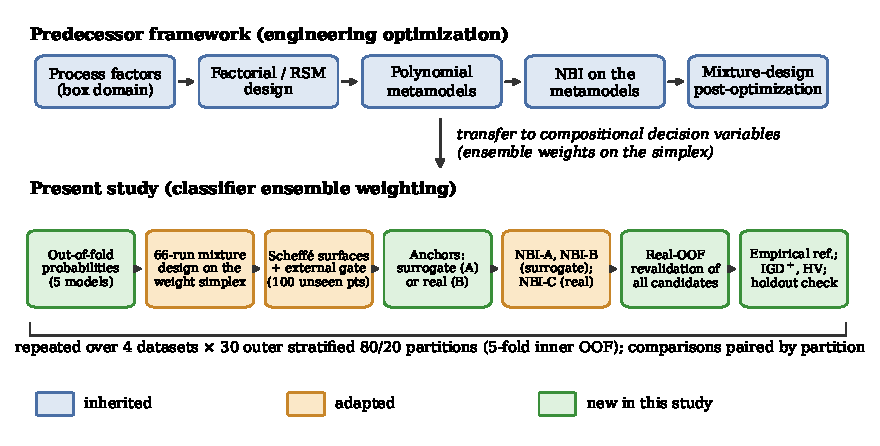
\includegraphics[width=\textwidth]{fig01_lineage_pipeline.pdf}
\caption{The predecessor DoE--RSM--NBI framework (top) and its transfer to classifier ensemble weighting (bottom).
Blue: inherited. Orange: adapted because the decision variables are compositional and the responses are
machine-learning metrics. Green: introduced in this study.}
\label{fig:pipeline}
\end{figure}

\subsection{The ensemble-weighting problem is a mixture problem}
\label{sec:method:problem}

Let $M$ probabilistic base classifiers produce estimates $p_1(x),\dots,p_M(x) \in [0,1]$ for a sample $x$. A
weighted soft-voting ensemble predicts
\begin{equation}
p_{\wvec}(x) \;=\; \sum_{i=1}^{M} w_i\, p_i(x) \;=\; \mathbf{P}\wvec ,
\label{eq:ensemble}
\end{equation}
where $\mathbf{P} \in [0,1]^{n \times M}$ collects the base-model probabilities for $n$ samples. For
$p_{\wvec}(x)$ to remain a probability for every input, the weights must satisfy
\begin{equation}
w_i \ge 0 \quad (i = 1,\dots,M), \qquad \sum_{i=1}^{M} w_i = 1 ,
\label{eq:simplex}
\end{equation}
that is, $\wvec \in \simplex$, the unit simplex in $\mathbb{R}^{M}$ and the canonical constraint set of a
\emph{mixture experiment}: the components are the classifiers, the vertices are single models used alone, and the
centroid is uniform soft voting. The sum-to-one constraint makes an intercept model singular, so the formalism is the
mixture design with a Scheff\'e canonical polynomial, not a factorial design. This correspondence, rather than any
performance argument, is why the framework transfers at all.

Three objectives are considered, all functions of $\wvec$ through \cref{eq:ensemble}:
\begin{align}
f_1(\wvec) &= -\operatorname{AUC}\!\left(y, \mathbf{P}\wvec\right) && \text{(discrimination, maximized)},\\
f_2(\wvec) &= \frac{1}{n}\sum_{k=1}^{n}\Big[-y_k \log p_{\wvec}(x_k) - (1-y_k)\log\!\big(1-p_{\wvec}(x_k)\big)\Big] && \text{(calibration, minimized)},\\
f_3(\wvec) &= c(\wvec) && \text{(inference cost, minimized)}.
\end{align}
The log-loss $f_2$ is convex and smooth in $\wvec$, whereas the area under the ROC curve is a rank statistic: $f_1$ is
piecewise constant in $\wvec$.

\subsection{Two cost models: a relaxation and a deployment cost}
\label{sec:method:cost}

Let $c_i$ be the measured inference cost of model $i$ (\cref{sec:protocol:models}). Deployment cost is a step
function: a model receiving \emph{any} non-negligible weight must be loaded and executed, one receiving none costs
nothing, giving the \emph{support cost}
\begin{equation}
c_{\mathrm{sup}}(\wvec) \;=\; \sum_{i=1}^{M} c_i \,\mathbf{1}\!\left[w_i > \varepsilon\right], \qquad \varepsilon = 10^{-3},
\label{eq:supportcost}
\end{equation}
which is discontinuous; every optimizer here instead sees the continuous relaxation
\begin{equation}
c_{\mathrm{w}}(\wvec) \;=\; \sum_{i=1}^{M} w_i c_i ,
\label{eq:weightedcost}
\end{equation}
the natural linear mixture response, which coincides with $c_{\mathrm{sup}}$ at the vertices but not on the
interior. We therefore optimize \cref{eq:weightedcost} and score the \emph{same} solutions under
\cref{eq:supportcost}, reporting every comparison under both; \cref{sec:results:cost} shows that the choice changes
which method wins. Because each $c_i$ is timed separately, including that model's own preprocessing,
\cref{eq:supportcost} is the time to run the active members one after another; it excludes model loading, and
parallel execution or preprocessing shared between members would give a different cost (\cref{sec:limitations}).

\subsection{Mixture design and Scheff\'e surrogates}
\label{sec:method:scheffe}

\paragraph{Design.} With $M = 5$ the design is a fixed 66-run mixture design, enumerated in supplementary
Section~S1, with points on the 5 pure vertices, all 10 binary edges, the ternary and quaternary faces and uniform
voting: the surrogate is supported on every face a sparse ensemble could occupy.

\paragraph{Models.} For a response $y$ the Scheff\'e canonical polynomials of order $1$, $2$ and the special cubic are
\begin{align}
\text{linear:}\quad & \hat y = \sum_i \beta_i w_i, \\
\text{quadratic:}\quad & \hat y = \sum_i \beta_i w_i + \sum_{i<j} \beta_{ij} w_i w_j, \label{eq:scheffequad}\\
\text{special cubic:}\quad & \hat y = \sum_i \beta_i w_i + \sum_{i<j} \beta_{ij} w_i w_j + \sum_{i<j<k} \beta_{ijk} w_i w_j w_k,
\end{align}
fitted by ordinary least squares without an intercept and without pure quadratic terms, which $\sum_i w_i = 1$ makes
redundant. No term elimination is performed: the canonical form is kept intact, so $\beta_i$ remains the predicted
response at vertex $i$.

\paragraph{External validation and the reliability gate.} Each replication also evaluates 100 Dirichlet compositions
outside the design, never used for fitting (supplementary Section~S1), giving an external $\rext$ and Spearman
$\rho_{\mathrm{ext}}$. \emph{Order selection} uses a parsimony rule --- the
lowest order whose external RMSE is within 10\% of the best --- so it is driven by out-of-design accuracy rather than
in-sample fit. The \emph{same} 100 compositions serve both steps, so the gate is not independent of order selection
--- the order it judges was chosen to do well on exactly these points --- and its pass rate should be read as an
optimistic estimate of out-of-design adequacy. Because $\rext$ is ill-posed on a nearly flat surface --- its
denominator is the variance of an almost constant response --- \cref{tab:gate} also reports the external RMSE of the
selected surface in the response's own units against the observed range over the same 100 points, the more
informative adequacy measure there. \emph{Admissibility} uses a \emph{reliability gate} whose thresholds
were fixed and committed to version control before the replicated benchmark was run, and never adjusted afterwards: a
surface is reliable only if
\begin{equation}
\rext \ge 0.5 \quad\text{and}\quad \rho_{\mathrm{ext}} \ge 0.9 .
\label{eq:gate}
\end{equation}
We describe this as pre-specification rather than preregistration: there is no
external registry entry, and the evidence is the version-controlled commit history. No source is cited for the two
thresholds: they are a convention chosen for this study, set before the replicated benchmark was run and not
calibrated on its results, although a single-dataset Santander pilot run had been completed before they were
committed. \Cref{tab:gate} reports the median $\rext$ and $\rho_{\mathrm{ext}}$ beside each pass
count, so that their distance from the thresholds can be read directly. The gate is a hypothesis under
test, not a filter applied to the results: surrogate-based optimization is run and reported \emph{regardless} of the
gate outcome, so that its predictive value can be measured (\cref{sec:results:anchors}; supplementary Section~S6).

\subsection{Normal Boundary Intersection on the simplex}
\label{sec:method:nbi}

NBI \citep{das1998nbi} was introduced to obtain a distributed representation of the Pareto boundary
(\cref{sec:rel:lineage}). Whether that distribution survives the map into revalidated objective space is one of the
questions this paper tests, and \cref{sec:results:metamodelfree} reports that in our setting it does not. For $m$
objectives $F = (F_1,\dots,F_m)$ the payoff matrix $\Phi$ has columns $F(\wvec^{*(k)})$ for the minimizers
$\wvec^{*(k)}$ of each $F_k$; its diagonal is the utopia point, and objectives are normalized by the utopia and
pseudo-nadir points extracted from $\Phi$. With $\bar\Phi$ the normalized payoff matrix and
$\hat{n} = -\bar\Phi\mathbf{1}$ the quasi-normal direction, each $\beta$ on the unit simplex of
\emph{scalarization} weights defines the subproblem
\begin{equation}
\max_{\wvec,\,t} \; t \quad \text{s.t.} \quad \bar\Phi\beta + t\,\hat{n} = \bar F(\wvec), \quad \wvec \in \simplex .
\label{eq:nbi}
\end{equation}
The simplex constraint is eliminated by optimizing over $M-1$ free variables with
$w_M = 1 - \sum_{i<M} w_i$, with a deterministic feasibility-recovery step for iterates that leave the simplex: the
free variables are clipped to $[0,1]$ and, if they still sum above one, renormalized onto the face $w_M = 0$. This is
a documented repair, not a Euclidean projection onto the simplex, and a candidate recovered this way is flagged
infeasible and excluded from the certified set. Without it, subproblems near a vertex terminate outside the feasible
region. For vertex values of $\beta$ the solution is the corresponding anchor, returned directly rather than
re-derived. All variants solve 66 subproblems per replication on the same $\beta$ lattice, so the arms are
compared at identical points of the CHIM.

\paragraph{The three variants.} The variants are defined by two methodological factors --- the source of the
objectives and the source of the anchors:

\begin{center}
\footnotesize
\setlength{\tabcolsep}{4pt}
\begin{tabular}{llll}
\toprule
Variant & Objectives in \cref{eq:nbi} & Anchors / payoff matrix & Real evaluations, standalone \\
\midrule
NBI-A & Scheff\'e surfaces & optima of the Scheff\'e surfaces & $1.7\times10^{2}$ \\
NBI-B & Scheff\'e surfaces & real out-of-fold optima & $\approx 4.1\times10^{4}$ \\
NBI-C & real out-of-fold objectives & real out-of-fold optima & $\approx 4.6\times10^{5}$ \\
\bottomrule
\end{tabular}
\end{center}

NBI-A is the lineage construction: everything, including the payoff matrix, comes from the metamodel. NBI-B changes
only the anchors, which become the real optima of \cref{sec:method:refs}; NBI-C removes the metamodel entirely.
Here and below, a \emph{real} anchor or optimum is one computed directly on the out-of-fold objectives of the training
part (\cref{sec:protocol:models}) rather than read off a Scheff\'e surface.
The last column charges every variant for the real evaluations it needs \emph{standalone}, each arm carrying the
stages it depends on rather than its solver stage alone (itemized in \cref{tab:compute}); design, gate and
ROC-AUC-search entries count evaluated compositions, whereas NBI-C's solve counts each ROC-AUC and each log-loss
computation separately, two per weight-vector evaluation. Real anchors are not free: NBI-B consumes about
$4\times10^{4}$ real evaluations that NBI-A does not (the direct ROC-AUC search of \cref{sec:method:refs}), and
its standalone wall clock is $1.2$--$12.7$ times NBI-A's.
Because $f_1$ is piecewise constant, NBI-C uses finite-difference steps of $10^{-3}$, multistart on the simplex, and
accepts an iterate whose equality residual is below $10^{-3}$ even without certified optimality,
whereas NBI-A and NBI-B optimize smooth polynomials and require full certification by sequential least-squares
quadratic programming \citep[SLSQP;][]{kraft1988software}, as implemented in SciPy \citep{virtanen2020scipy}. This asymmetry follows from
the objective, not from tuning, and it bounds the causal reading. A versus B is not a single-factor contrast:
replacing the anchors simultaneously moves the utopia point, rescales both normalization axes through the payoff
matrix, reorients the CHIM and every quasi-normal direction, and---because the three vertex values of $\beta$ return
their anchor directly---substitutes three returned candidates. \Cref{sec:results:anchors} separates the last of these
from the rest. B versus C tests removal of
\emph{surrogate error in the interior} once real anchors are supplied, but is not a perfectly identical numerical
experiment, because changing the objective from a smooth polynomial to a piecewise-constant rank statistic
necessarily changes solver semantics. Solver outcomes are therefore reported separately for each arm
(supplementary Section~S7).

\subsection{References, comparators and revalidation}
\label{sec:method:refs}

\paragraph{Single-objective references.} Each replication computes seven single-objective references, tabulated in
supplementary Section~S2: best single model, uniform voting, logistic stacking, the SLSQP log-loss optimum (convex,
hence global), a derivative-free ROC-AUC optimum over $4\times10^{4}$ sampled compositions with local refinement, and
the two Scheff\'e-surface optima. The log-loss and AUC optima double as the real anchors of NBI-B
and NBI-C. SLSQP on the convex log-loss remains the correct tool for the single-objective problem; NBI is not
proposed as a replacement for it.

\paragraph{Comparators.} Two cheap alternatives run on every replication: random weighted scalarization, which
draws 66 scalarization weight vectors from $\mathrm{Dirichlet}(\mathbf{1})$ and minimizes the weighted sum of the
\emph{same} Scheff\'e surfaces with the same real anchors as NBI-B; and a 66-point random
$\mathrm{Dirichlet}(\mathbf{1})$ sample of the weight simplex. The second is matched to the NBI sets only in the
\emph{number of returned candidates} and is not compute-matched; it is a floor check on the geometry of the reference
front, not an efficiency baseline.

\paragraph{Revalidation.} Every candidate from every method --- the three NBI arms, both comparators, the 66 design
runs and the references --- is re-evaluated on the exact out-of-fold objectives, and non-dominated filtering applied
to those revalidated values, before any indicator is computed. No result in this paper is read off a surrogate.

\subsection{Empirical Pareto reference and quality indicators}
\label{sec:method:reference}

The true Pareto set of \cref{eq:ensemble} over $\simplex$ is unknown, so each replication constructs an
\emph{empirical Pareto reference}: at least $10^{5}$ compositions
from $\mathrm{Dirichlet}(\mathbf{1})$ and $\mathrm{Dirichlet}(0.3\cdot\mathbf{1})$ in equal parts, augmented with the
simplex lattice, all vertices and edges, and a 40-cap $\varepsilon$-constraint sweep, evaluated on the real objectives
and filtered to the non-dominated set. An independent sample of $2\times10^{4}$ points checks convergence: if it
displaces more than 5\% of the front, the reference is enlarged and rechecked, up to three rounds (per-dataset
convergence diagnostics in supplementary Section~S8). This sampled core
contains no output of the five methods compared in this study --- NBI-A, NBI-B, NBI-C, random weighted scalarization
and NSGA-II. It is not, however, free of optimization output: it carries the 40 $\varepsilon$-constraint solutions and
the seven single-objective references of \cref{sec:method:refs}, among them the real ROC-AUC and log-loss optima that
NBI-B and NBI-C receive as anchors and the two Scheff\'e-surface optima that NBI-A receives. On Santander the
$\varepsilon$-constraint sweep supplies a median of 38 of the roughly 135 core-front points and the single-objective
references a median of 4 (\texttt{tables/reference\_diagnostics.csv}). The final reference used for scoring is the non-dominated union of that core with every candidate set, making it
at least as good as any method scored against it.

We call this an empirical reference, never a true Pareto front: it is a sample-based upper bound, and because
candidate sets contribute to it, a method contributing many points is partly graded against itself.

Approximation sets are scored on min--max normalized objectives. The two primary endpoints are $\igdp$
\citep{ishibuchi2015modified} and the exact hypervolume with reference point $1.1$ on each axis, expressed as a ratio
to the reference hypervolume \citep{zitzler1999multiobjective}; generational distance
\citep{vanveldhuizen2000multiobjective}, inverted generational distance, Schott spacing \citep{schott1995fault},
coverage and the joint non-dominated fraction \citep{zitzler2003performance} are defined and reported for every set
in supplementary Section~S4.

\subsection{The normalization box}
\label{sec:method:normbox}

Every indicator is computed on objectives mapped into $[0,1]$ by one box, and the box is not a fixed property of the
problem. Let $\mathcal{F}$ be the empirical reference front of the replication --- the sampled core united with every
candidate set --- under one of the two cost definitions. The box is the componentwise minimum and maximum of $\mathcal{F}$:
\begin{equation}
\ell_k \;=\; \min_{F \in \mathcal{F}} F_k, \qquad u_k \;=\; \max_{F \in \mathcal{F}} F_k, \qquad
\tilde F_k \;=\; \frac{F_k - \ell_k}{u_k - \ell_k}, \qquad k = 1,2,3 .
\label{eq:normbox}
\end{equation}
Three consequences follow, and each constrains how the numbers in \cref{sec:results} may be read.

\emph{(i) Within a replication the box is common to every arm.} All candidate sets of a replication are scored under
the same $\ell$ and $u$, so the paired contrast between two arms is a difference of commensurable quantities and no
arm is scored on a box of its own. The contrast is not, however, invariant to the box: the hypervolume ratio depends
on the box only through the raw reference point $u + 0.1\,(u-\ell)$, and $\igdp$ is computed on axes rescaled by
$1/(u_k-\ell_k)$, so a different box can change a contrast's magnitude and, between sets that do not dominate one
another, its sign. Nor is the box independent of the arms, whose candidates can dominate the core points that set a
bound (\cref{sec:results:cost}).

\emph{(ii) The reference, and with it the box, changes when a method is added,} because a new candidate set can add
points to $\mathcal{F}$ and remove points it dominates; this changes the reference hypervolume and the $\igdp$
reference set and can widen or narrow the box. Adding the NSGA-II arm moves median levels slightly: on identical
candidate sets NBI-C's median hypervolume ratio is $0.989$, $0.983$, $0.982$ and $0.976$ without NSGA-II in the
reference (\cref{sec:results:metamodelfree}) and $0.990$, $0.981$, $0.981$ and $0.977$ with it (\cref{tab:nsga2}).
Single partitions move more than the medians, and a paired contrast close to zero can change direction when a method
is added. Absolute indicator levels, and paired differences close to zero, are therefore only interpretable together
with the set of methods that built the reference; for this reason the NSGA-II comparison is also scored against the
sample core, which contains no output of the five compared methods and does not change when one is added
(\cref{sec:results:nsga2}).

\emph{(iii) The box differs between replications,} since each replication has its own reference front. Absolute
levels are comparable within a replication but not across partitions, and a mean of $\Delta\hv$ over 30 partitions is
a mean over 30 different scales. Each paired difference is computed within a single box, which is why medians, win
counts and per-partition distributions are reported alongside means, although a partition with an unusual box can
still change a win count through consequence (i); \cref{sec:results:cost} withdraws one earlier between-partition
reading that this rescaling, not the optimizers, produced.

\section{Experimental protocol}
\label{sec:protocol}

The computational protocol (partitions and seeds, base models, design, surfaces and gate thresholds, optimizers and
scoring) was committed to version control before the replicated study was launched with the planned ten
replications per dataset. Its only change during execution was a solver-robustness fix after a crash in
replication~0; the replication-0 stages completed before the fix were kept, and the part of the change that can be
checked on the stored surfaces moves no stored solution by more than $10^{-10}$ in any weight (supplementary Section~S1). After the ten-replication
analysis had been completed and reported, the study was extended to 30 replications, reusing the computational
protocol without modification, and \cref{sec:results:r30} reports what that extension changed. The NSGA-II baseline
(\cref{sec:results:nsga2}) was added after the 30-replication analysis, with its configuration committed before its
first run.

\subsection{Datasets}
\label{sec:protocol:data}

Four public binary tabular classification problems span prevalence, dimensionality and feature type
(\cref{tab:datasets}): Santander \citep{kagglesantander} (high-dimensional, anonymized, numeric, 10\% positives);
BNP Paribas \citep{kagglebnp} (numeric plus high-cardinality categorical features, 76\% positive); Porto Seguro
\citep{kaggleporto} (strongly imbalanced at 3.6\% positives, subsampled to 200{,}000 rows by a single stratified
draw with a recorded seed to bound runtime); and UCI credit default \citep{yeh2009ucidataset} (small and
low-dimensional). For the three Kaggle competition datasets the competition test labels are not
public and were never used: all training, weighting, thresholding and model selection use only the published training
file, from which every performance figure in this paper is derived.

\begin{table}[t]
\centering
\caption{Datasets. Rows used, number of raw features, positive-class prevalence and training/holdout sizes of each outer partition (stratified 80/20). Kaggle test labels are never used; all selection uses 5-fold out-of-fold predictions within the training part. $^{\dagger}$200,000-row stratified subsample of the 595,212 available rows, drawn once with a recorded seed.}
\label{tab:datasets}
\small
\resizebox{\textwidth}{!}{%
\begin{tabular}{llrrrl}
\toprule
Dataset & Source & Rows & Features & Prevalence & Train / holdout rows \\
\midrule
Santander & Santander Customer Transaction (Kaggle 2019) & 200,000 & 200 & 0.100 & 160,000 / 40,000 \\
BNP Paribas & BNP Paribas Cardif Claims (Kaggle 2016) & 114,321 & 131 & 0.761 & 91,456 / 22,865 \\
Porto Seguro & Porto Seguro Safe Driver (Kaggle 2017)$^{\dagger}$ & 200,000 & 57 & 0.036 & 160,000 / 40,000 \\
UCI credit & Default of credit card clients (UCI id 350) & 30,000 & 23 & 0.221 & 24,000 / 6,000 \\
\bottomrule
\end{tabular}}
\end{table}


\subsection{Base models and leakage control}
\label{sec:protocol:models}

The ensemble contains $M = 5$ deliberately heterogeneous learners with fixed hyperparameters and no hyperparameter
search: $\ell_2$-regularized logistic regression; Gaussian naive Bayes; $k$-nearest neighbours with $k = 100$; a
random forest with 200 trees and a minimum of 20 samples per leaf; and gradient-boosted trees (XGBoost, 400 rounds,
depth 6, learning rate 0.1, subsample and column subsample 0.8) \citep{chen2016xgboost}. The first four are the
\texttt{scikit-learn} implementations \citep{pedregosa2011scikit}. These values were committed to the project code on
2026-07-06, before the replicated study, and were not changed afterwards; Gaussian naive Bayes uses the library
defaults, as do the inverse regularization strength of logistic regression ($C = 1$) and the XGBoost depth. The zoo
spans the accuracy--cost--calibration space rather than forming a competitive stack: Gaussian naive Bayes is the best
member out of fold on Santander but has the worst log-loss on the other three datasets, and $k$-nearest neighbours,
the weakest member by ROC-AUC on Santander and Porto Seguro, costs more at inference time than the other four
combined (supplementary Section~S2; implications in \cref{sec:limitations}). Preprocessing (imputation,
standardization and encoding, detailed per model in supplementary Section~S1) is fitted inside each training fold and
never on validation data.

Each replication splits the dataset by a stratified 80/20 partition into a training part and an untouched holdout.
Within the training part, stratified 5-fold cross-validation produces out-of-fold probability estimates $\mathbf{P}$
for all five models; these are the only quantities the design, the surfaces, the optimizers and the selection rules
ever see. Each model is then refitted once on the whole training part to produce holdout probabilities $\mathbf{Q}$,
used exclusively for the confirmation analysis of \cref{sec:results:holdout}. Every entry of $\mathbf{P}$ and
$\mathbf{Q}$ is clipped to $[10^{-3}, 1-10^{-3}]$, a constant fixed before the study and never changed: $k$-nearest
neighbours with $k = 100$ outputs exact zeros and ones, which can make the log-loss infinite at its vertex, and
clipping the components rather than the blend keeps \cref{eq:ensemble} linear in $\wvec$. Because \cref{eq:ensemble} is linear in
$\wvec$, evaluating any weight vector costs one matrix--vector product, which is what makes an empirical reference of
$10^{5}$ points and a metamodel-free NBI arm affordable.

Inference cost $c_i$ is measured, not assumed: per model and replication, the median wall-clock time of five
consecutive \texttt{predict\_proba} calls of the refitted model, including preprocessing, in milliseconds per
1{,}000 rows. One batch of holdout rows, drawn with the replication seed, is shared by the five models (10{,}000 rows;
the whole 6{,}000-row holdout on UCI credit). The models are timed one after another in a fixed, non-randomized order
(logistic regression, Gaussian naive Bayes, $k$-nearest neighbours, random forest, XGBoost), each right after its own
refit, an untimed holdout prediction and an untimed warm-up call on the batch. Three of them ($k$-nearest neighbours,
the random forest and XGBoost) are set to use all 14 cores (\texttt{n\_jobs}~$=-1$); the code and the launch script
set no other parallel option or thread limit for the timed calls.

\subsection{Replication, seeds and the statistical unit}
\label{sec:protocol:replication}

The entire pipeline, from the outer partition through scoring, is executed $R = 30$ times per dataset, giving 120
replications, with the outer partition, the inner folds and every stochastic component seeded by
$\text{20260904} + r$ for replication $r$. All seeds are persisted in the manifest, and the checkpointed runner
described in the Reproducibility statement recomputes any stage exactly, except that re-running the out-of-fold stage
re-measures the wall-clock costs $c_i$ and therefore changes every result that depends on them.

The statistical unit is \textbf{one outer partition of one dataset}. Because all methods are evaluated on the same
partition, every comparison is \emph{paired}. Two consequences constrain the analysis throughout.

First, the 30 partitions of a dataset overlap heavily: two independent stratified 80/20 draws have an expected
intersection of $0.8 \times 0.8 = 64\%$ of the dataset, which is $80\%$ of each training part, a Jaccard index of
two-thirds. Any two training parts therefore share most of their rows.
The replication distribution therefore measures \emph{sensitivity to data partitioning}, not sampling from a
population, and the effective information is far below 30 independent runs. Second, and consequently, the dataset is
the unit of generalization: results are summarized per dataset and the four dataset-level results are then compared.
Nothing is pooled across the $4 \times 30$ replications, and no statement of the form ``$N = 120$ independent
experiments'' is made anywhere in this paper.

\subsection{Statistical analysis}
\label{sec:protocol:stats}

The statistical analysis plan (supplementary Section~S1) designates four primary comparisons. NBI-B versus NBI-A and
NBI-C versus NBI-B address RQ4 and RQ5. NBI-C versus random scalarization and NBI-C versus the random Dirichlet sample
compare NBI-C, as specified and not at equal budget, with the two cheap alternatives of \cref{sec:method:refs}: the
first comparison is confounded with the objective source and the second is a floor check. The plan was committed to
version control after the first ten replications had been run and analysed, minutes after the extension to 30
replications was launched and before any of its partitions had been completed, so it is prospective only for
partitions 10--29. The paired contrasts coded before the benchmark produced its first output were descriptive and
compared both cheap alternatives with NBI-B rather than NBI-C; \cref{sec:results:metamodelfree} reports both
pairings. The
primary endpoints are $\igdp$ and the hypervolume ratio, computed on the revalidated \emph{out-of-fold objectives of
the 80\% training part} (the only quantities the design, the surfaces, the optimizers and the selection rules ever
see; \cref{sec:protocol:models}) against the empirical reference of the same replication, under the weighted cost
that the optimizers actually minimized; the support-cost repetition is a sensitivity analysis. The
untouched 20\% holdout enters no primary endpoint: it is used only for the confirmation analysis of
\cref{sec:results:holdout}. The primary endpoints therefore measure how well a returned front approximates the
empirical front on the training part's out-of-fold objectives, not how a front generalizes; only the holdout
transfer bears on generalization, and it scores one selected solution per set. All other indicators are descriptive.

Paired differences are signed so that $\Delta > 0$ always favours the first-named (new) method:
$\Delta\hv = \hv_{\text{new}} - \hv_{\text{ref}}$ and
$\Delta\igdp = \igdp_{\text{ref}} - \igdp_{\text{new}}$. For each dataset $\times$ comparison $\times$ endpoint we
report the mean and median with percentile-bootstrap 95\% intervals (10{,}000 resamples, fixed seed), the quartiles
and range \citep{efron1993bootstrap}, the win/tie/loss counts with a tie tolerance of $10^{-4}$, the win fraction
with a Wilson 95\% interval \citep{wilson1927probable}, and the matched-pairs rank-biserial correlation
\citep{kerby2014simple} as a distribution-free effect size. These and all other replication-level intervals in this
paper treat the replications of a dataset as independent observations: they describe partition sensitivity within
that dataset, carry no correction for partition overlap and do not by themselves establish significance.

An ordinary paired $t$-test on resampled partitions is anticonservative, so the primary test is the Nadeau--Bengio
corrected resampled $t$-test \citep{nadeau2003inference}: with $J = 30$ paired differences $d_j$,
\begin{equation}
t \;=\; \frac{\bar d}{\sqrt{\operatorname{var}(d)\left(\tfrac{1}{J} + \rho\right)}}, \qquad
\rho \;=\; \frac{n_{\text{test}}}{n_{\text{train}}} \;=\; \frac{0.20}{0.80} \;=\; 0.25,
\label{eq:nb}
\end{equation}
on $J - 1$ degrees of freedom. The correction inflates the variance by a factor of
$(1/30 + 0.25)/(1/30) \approx 8.5$, multiplying standard errors by about 2.9 relative to the naive test. One caveat
attaches to $\rho$ and we state it plainly: the heuristic $\rho = n_{\text{test}}/n_{\text{train}}$ was derived for a
statistic measured on the held-out portion of each resample, whereas both primary endpoints here are measured on the
training part, whose rows two replications share to the extent computed above. The value $\rho = 0.25$ is therefore
an assumed correction, not an estimate of the correlation between replications, which was not measured; the
training-part overlap suggests that it may understate that correlation, in which case the corrected test would
still be anticonservative. Every significance statement below holds \emph{at} the assumed $\rho = 0.25$, and the
effect sizes, the paired direction counts and their spread over partitions, which do not depend on $\rho$, are the
primary evidence and are reported alongside it. Within each
dataset the eight primary tests form one family and receive a Holm correction \citep{holm1979simple}; no correction
is applied across datasets, because datasets are not pooled. A Wilcoxon signed-rank test
\citep{wilcoxon1945individual} is reported alongside as a distribution-free check, but it is not corrected for overlap and cannot rescue a non-significant corrected result.

Where a paired-difference distribution is visibly bimodal or heavy-tailed, the mean-based test is uninformative by
construction and we say so, reporting the median with its bootstrap interval, the win fraction with its Wilson
interval and the rank-biserial correlation as descriptive evidence of consistency instead. Throughout, effect consistency takes precedence
over $p$-values. Frequencies over replications are reported with Wilson and Jeffreys 95\% intervals \citep{brown2001interval}.

\section{Results}
\label{sec:results}

Results are organized by research question, with per-claim provenance in the supplementary claims map. Indicators use
the weighted cost of \cref{eq:weightedcost} unless stated otherwise.

One fact frames the rest: weighting helps, but modestly. The log-loss optimum improves out-of-fold ROC-AUC over the
best single model by $0.0037$, $0.0056$, $0.0060$ and $0.0007$ --- one to two orders of magnitude more than the
differences between the multiobjective methods studied here.

\subsection{RQ1: Accuracy of the Scheff\'e surfaces}
\label{sec:results:gate}

\begin{table}[t]
\centering
\caption{Surrogate reliability over 30 partitions, all quantities measured on the \emph{same} 100 unseen
compositions: the parsimony rule selects the Scheff\'e order on them (lowest order within 10\% of the best external
RMSE) and the pre-specified reliability gate ($\rext \ge 0.5$ and Spearman $\rho_{\mathrm{ext}} \ge 0.9$) is then
scored on them, so the gate is not independent of order selection. Orders are abbreviated lin./quad./sp.\,cubic. Pass
counts carry Wilson 95\% intervals, and the median external $R^2$ is shown with the bootstrap interval of the mean
external $R^2$. The last two columns give the median external RMSE of
the selected surface in the response's own units and the median observed range of that response over the same 100
points: on a flat surface $\rext$ is ill-posed, so the RMSE read against the range is the more informative adequacy
measure. Sources: \texttt{statistics/reliability\_gate\_r30.csv}, \texttt{tables/scheffe\_orders.csv}.}
\label{tab:gate}
\small
\resizebox{\textwidth}{!}{%
\begin{tabular}{llllll r r r}
\toprule
Dataset & Response & Selected order (count) & Pass & Wilson 95\% & Median $\rext$ [95\% CI] & Median $\rho_{\mathrm{ext}}$ & RMSE$_{\mathrm{ext}}$ & Range \\
\midrule
Santander & ROC-AUC & quad. 26, lin. 4 & 0/30 & [0.00, 0.11] & -0.333 [-0.559, -0.199] & 0.830 & 0.0087 & 0.040 \\
Santander & log-loss & quad. 29, sp.\,cubic 1 & 30/30 & [0.89, 1.00] & 0.971 [0.967, 0.973] & 0.994 & 0.0028 & 0.081 \\
BNP Paribas & ROC-AUC & lin. 22, quad. 7, sp.\,cubic 1 & 5/30 & [0.07, 0.34] & 0.118 [-0.034, 0.244] & 0.908 & 0.0096 & 0.053 \\
BNP Paribas & log-loss & lin. 21, quad. 7, sp.\,cubic 2 & 3/30 & [0.03, 0.26] & -0.180 [-0.246, 0.042] & 0.955 & 0.1214 & 0.694 \\
Porto Seguro & ROC-AUC & quad. 26, sp.\,cubic 2, lin. 2 & 16/30 & [0.36, 0.70] & 0.519 [0.482, 0.581] & 0.924 & 0.0037 & 0.030 \\
Porto Seguro & log-loss & lin. 20, quad. 8, sp.\,cubic 2 & 12/30 & [0.25, 0.58] & 0.506 [0.492, 0.580] & 0.995 & 0.0582 & 0.448 \\
UCI credit & ROC-AUC & quad. 20, sp.\,cubic 10 & 30/30 & [0.89, 1.00] & 0.992 [0.989, 0.992] & 0.995 & 0.0015 & 0.077 \\
UCI credit & log-loss & quad. 27, sp.\,cubic 3 & 30/30 & [0.89, 1.00] & 0.993 [0.991, 0.993] & 0.993 & 0.0066 & 0.427 \\
\bottomrule
\end{tabular}}
\end{table}


\begin{figure}[t]
\centering
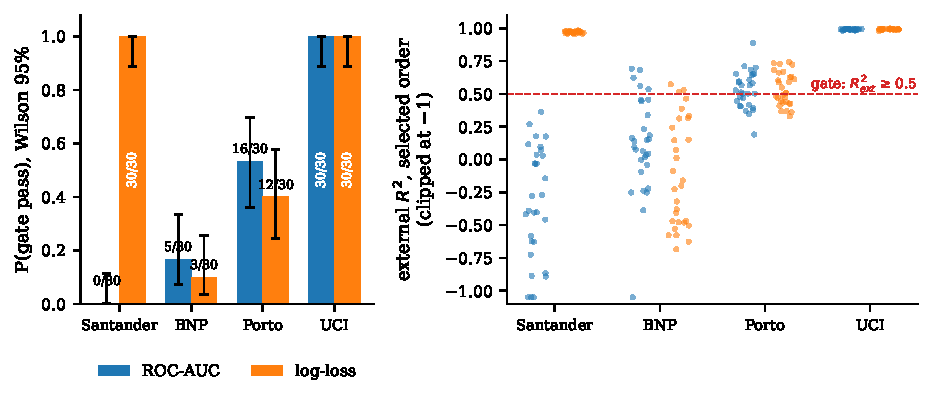
\includegraphics[width=\textwidth]{fig05_reliability_gate.pdf}
\caption{Left: reliability-gate pass frequency per dataset and response over 30 partitions, with Wilson 95\%
intervals. Right: the external $\rext$ of the selected order per partition; the dashed line is the gate's $\rext$
threshold, and because the gate also requires $\rho_{\mathrm{ext}} \ge 0.9$, some Porto Seguro points above it fail.
Within Santander the two responses fall on opposite sides of the gate.}
\label{fig:gate}
\end{figure}

Surrogate adequacy depends on dataset and response alike (\cref{tab:gate}, \cref{fig:gate}). The ROC-AUC surface
passes the gate in $0/30$ partitions on Santander, $5/30$ on BNP Paribas, $16/30$ on Porto Seguro and $30/30$ on UCI
credit; the log-loss surface passes in $30/30$, $3/30$, $12/30$ and $30/30$. Santander is sharpest: on the same
partition its log-loss surface is essentially exact while its ROC-AUC surface has \emph{negative} external $\rext$ ---
worse than predicting the mean --- even though its external rank correlation is a respectable $0.830$. Porto Seguro
sits on the threshold for both responses and 30 partitions do not resolve it either way --- a property of the problem,
not a sample-size deficiency.

The failures are misspecification, not extrapolation: the design contains all five vertices, so every validation
composition lies inside the convex hull of the design points. As an implementation check, the Brier score, which is
exactly quadratic in $\wvec$, is reproduced with $\rext = 1.000$ in all 120 replications; this confirms the fitting
code and the estimability of the quadratic model on this design, not the adequacy of the other surfaces
(\cref{fig:surrogate}).

\begin{figure}[t]
\centering
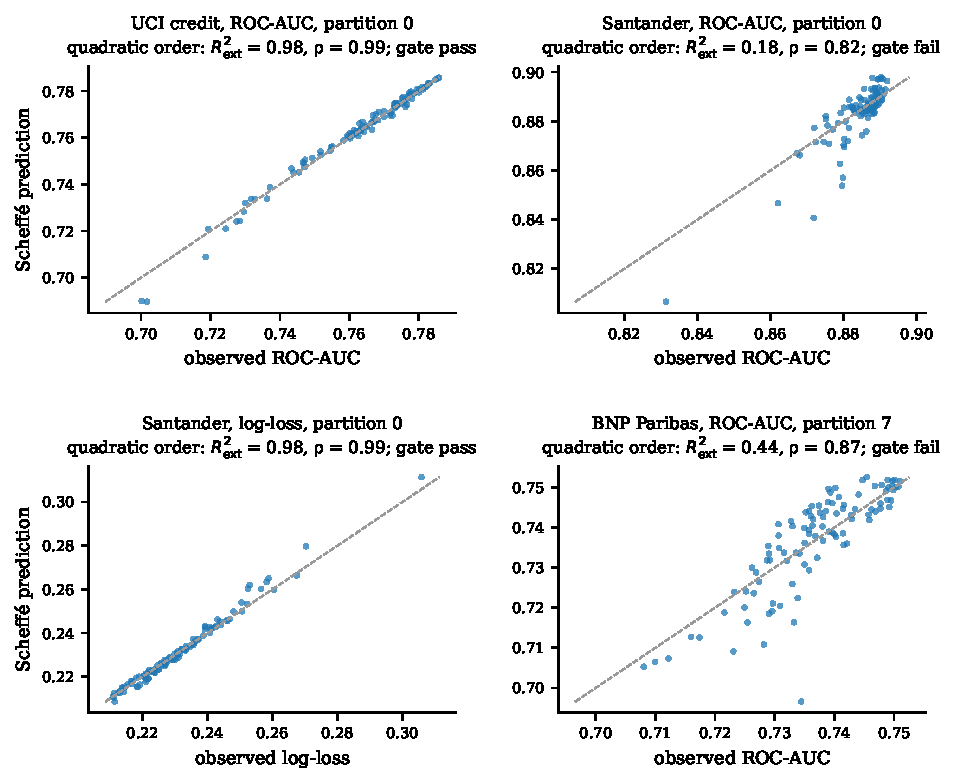
\includegraphics[width=\textwidth]{fig02_surrogate_validation.pdf}
\caption{Predicted versus observed response on the 100 unseen Dirichlet compositions of one partition, for four
dataset--response pairs spanning the regimes of \cref{tab:gate}. The dashed line is the identity.}
\label{fig:surrogate}
\end{figure}

\subsection{RQ2: Surface stability and what the coefficients mean}
\label{sec:results:coefficients}

The quadratic surfaces, fitted in every partition whatever order is selected there, are stable across resampling:
the four largest interaction coefficients keep their sign in all eight dataset--response cells, the largest-magnitude
term is the same at $R = 10$ and $R = 30$ in all eight and is the per-partition largest in seven of them, and its
between-partition coefficient of variation lies between $0.007$ and $0.17$ (per-cell detail in supplementary
Section~S3). These statistics measure sensitivity to data partitioning, not accuracy: the same 66-run design is used
in every replication and any two training parts share most of their rows (\cref{sec:protocol:replication}), so the
error of a misspecified surface, including any bias in its coefficients, recurs in every partition, and agreement
between partitions cannot reveal it. Santander shows the difference: the leading coefficients of its log-loss and
ROC-AUC surfaces both vary by about one percent between partitions (coefficients of variation $0.007$ and $0.011$),
yet the log-loss surface passes the gate in every partition and the ROC-AUC surface in none (\cref{tab:gate}).

Interpreting those coefficients requires the classical criterion
\citep{scheffe1958mixtures,cornell2002mixtures} stated correctly. The edge profile
$\hat y(t) = \beta_j + (\beta_i - \beta_j)t + \beta_{ij}t(1-t)$ implied by
\cref{eq:scheffequad} has an interior optimum above both pure components if and only if
\begin{equation}
\beta_{ij} \;>\; \lvert \beta_i - \beta_j \rvert
\label{eq:edgecond}
\end{equation}
(derivation in supplementary Section~S3), which already guards against the naive reading: a large $\beta_{ij}$ on an
edge joining two very unequal vertices need not beat the better one. Our finding is not that this criterion is
unknown, but that \emph{the fitted surfaces pass it and are still wrong}.

For the largest-$\beta$ pair of every dataset \cref{eq:edgecond} holds in all thirty partitions (\cref{tab:edge}), yet
on the real out-of-fold objectives the predicted superior blend materializes on one dataset only. The real 50/50 blend
is \emph{worse} than its better member in $30/30$ partitions on Santander, BNP Paribas and UCI credit, and beats both
members only on Porto Seguro ($30/30$; per-pair magnitudes in supplementary Section~S3); the untouched holdout repeats
this. Across all ten pairs of every dataset (\cref{tab:edge}) all 20 disagreements between the criterion and the real
50/50 blend are the surface predicting a superior blend that the midpoint mixture does not deliver; because the
criterion concerns the best point of an edge and this test only its midpoint, the tally overstates over-prediction and
cannot detect a superior real blend away from the midpoint.

\begin{table}[t]
\centering
\caption{The classical synergism criterion applied correctly, and what the real objectives say. On the binary edge
$i$--$j$ of a quadratic Scheff\'e model the fitted surface has an interior optimum exceeding both pure components if
and only if $\hat\beta_{ij} > |\hat\beta_i - \hat\beta_j|$. Columns 3--5 evaluate that criterion for the
largest-$\hat\beta$ pair of each dataset; column 6 gives the partitions in which the \emph{real} out-of-fold 50/50
blend of the same pair beats its better member. The last three columns compare the criterion with the real 50/50 blend
across all ten pairs: agreements, cases where the surface predicts a superior blend that the midpoint mixture does not
deliver, and the reverse. Because only the midpoint of each real edge is tested, the tally overstates over-prediction
and cannot detect a superior real blend elsewhere on the edge. Source: \texttt{tables/edge\_condition\_summary.csv}.}
\label{tab:edge}
\small
\setlength{\tabcolsep}{4pt}
\resizebox{\textwidth}{!}{%
\begin{tabular}{ll rr cc ccc}
\toprule
& & \multicolumn{3}{c}{Largest-$\hat\beta$ pair, fitted surface} & Real blend & \multicolumn{3}{c}{All 10 pairs} \\
\cmidrule(lr){3-5}\cmidrule(lr){6-6}\cmidrule(lr){7-9}
Dataset & Pair & $\hat\beta_{ij}$ & $|\hat\beta_i - \hat\beta_j|$ & criterion met & beats better member & agree & surface over-predicts & under-predicts \\
\midrule
Santander & GNB$\cdot$kNN & 0.243 & 0.130 & 30/30 & 0/30 & 6/10 & 4 & 0 \\
BNP Paribas & GNB$\cdot$XGB & 0.148 & 0.110 & 30/30 & 0/30 & 4/10 & 6 & 0 \\
Porto Seguro & GNB$\cdot$kNN & 0.071 & 0.025 & 30/30 & 30/30 & 7/10 & 3 & 0 \\
UCI credit & GNB$\cdot$XGB & 0.130 & 0.100 & 30/30 & 0/30 & 3/10 & 7 & 0 \\
\bottomrule
\end{tabular}}
\end{table}


The mechanism is visible in \cref{fig:beta}: the largest interaction attaches to the \emph{weakest} vertex of the pair
(\cref{tab:edge}) and tracks the pair's vertex-quality gap (supplementary Section~S3). Consistently, the pairs whose
real blend does beat its better member in at least 80\% of partitions are different, smaller-$\beta$ pairs on every
dataset except Porto Seguro (supplementary Section~S3).

The criterion is correct and should be applied through \cref{eq:edgecond} rather than by reading the sign of
$\beta_{ij}$, but on these ensembles it inherits the misspecification of the surface it is computed from and must be
confirmed on the real objective, at the cost of one matrix product per pair, before a pair is called complementary.
Log-loss interaction signs are uninformative: log-loss is convex in $p_{\wvec}$, so by Jensen's inequality a real blend
never lies above its chord, yet the fitted surfaces give the six pairs without Gaussian naive Bayes stable
\emph{positive} log-loss interactions on BNP Paribas and Porto Seguro (supplementary Section~S3 and
\texttt{statistics/\allowbreak coefficient\_\allowbreak stability\_\allowbreak r30.csv}). The ROC-AUC signs are
interpretable, but what the blend test contradicts is not their sign: it is the reading of a large $\beta_{ij}$, through
\cref{eq:edgecond}, as a blend that beats its better member.

\begin{figure}[t]
\centering
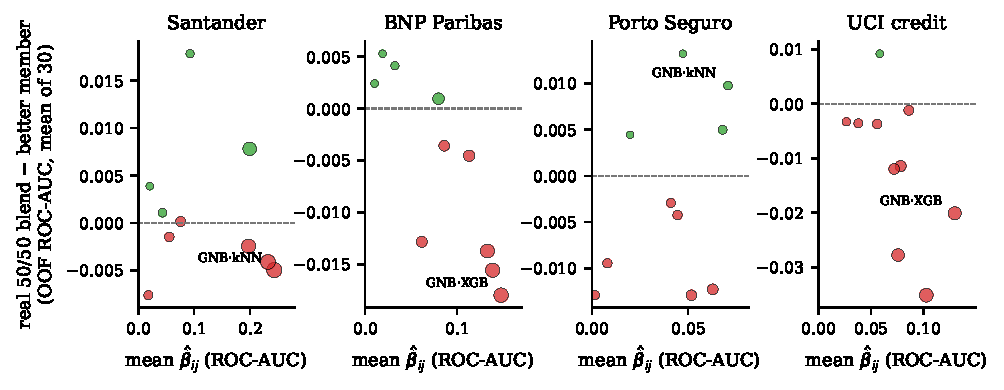
\includegraphics[width=\textwidth]{fig07_beta_vs_synergy.pdf}
\caption{Fitted interaction coefficient against the real gain of the corresponding 50/50 blend over its better member,
one point per classifier pair, averaged over 30 partitions; marker size is the vertex-quality gap. Green markers
denote pairs whose blend wins in at least 80\% of partitions; the largest-$\beta$ pair is labelled.}
\label{fig:beta}
\end{figure}

\subsection{RQ3 and RQ4: Surrogate versus real anchors}
\label{sec:results:anchors}

\begin{table*}[t]
\centering
\caption{Primary paired comparisons under the weighted cost, 30 partitions per dataset. $\Delta > 0$ favours the
first-named (new) set ($\Delta\mathrm{IGD}^+ = \mathrm{IGD}^+_{\mathrm{ref}} - \mathrm{IGD}^+_{\mathrm{new}}$,
$\Delta\mathrm{HV} = \mathrm{HV}_{\mathrm{new}} - \mathrm{HV}_{\mathrm{ref}}$). Median with its percentile-bootstrap
95\% interval (not corrected for partition overlap), wins/ties/losses, and the Holm-corrected Nadeau--Bengio
significance band ($\rho = 0.25$, family of eight tests per dataset; \emph{n.s.} means the corrected test does not
reach 0.05, which for a bimodal or heavy-tailed difference is expected and is why the median and the win count are
reported). Each dataset's eight-test family also contains NBI-C versus random scalarization (confounded with the
objective source) and NBI-C versus the random Dirichlet sample (a floor check); those comparisons, the means,
rank-biserial effect sizes, exact $p$-values and the full support-cost repetition are in supplementary Section~S5. Source:
\texttt{statistics/paired\_primary\_effects.csv}, \texttt{paired\_primary\_tests.csv}.}
\label{tab:paired}
\small
\setlength{\tabcolsep}{4pt}
\resizebox{\textwidth}{!}{%
\begin{tabular}{ll lcc lcc}
\toprule
& & \multicolumn{3}{c}{$\Delta \mathrm{IGD}^+$} & \multicolumn{3}{c}{$\Delta$ hypervolume ratio} \\
\cmidrule(lr){3-5}\cmidrule(lr){6-8}
Dataset & Comparison & median [95\% CI] & W/T/L & Holm $p$ & median [95\% CI] & W/T/L & Holm $p$ \\
\midrule
Santander & NBI-B vs NBI-A & +0.125 [+0.086, +0.145] & 30/0/0 & $<$0.01 & +0.196 [+0.143, +0.216] & 30/0/0 & $<$0.01 \\
 & NBI-C vs NBI-B & +0.0017 [+0.0011, +0.0020] & 28/0/2 & n.s. & +0.0084 [+0.0072, +0.0093] & 28/0/2 & $<$0.01 \\
\addlinespace
BNP Paribas & NBI-B vs NBI-A & +0.0146 [+0.0136, +0.0172] & 30/0/0 & n.s. & +0.058 [+0.051, +0.070] & 30/0/0 & n.s. \\
 & NBI-C vs NBI-B & -0.0028 [-0.0044, -0.0015] & 6/0/24 & n.s. & +0.0106 [+0.0087, +0.0128] & 24/0/6 & n.s. \\
\addlinespace
Porto Seguro & NBI-B vs NBI-A & +0.0296 [+0.0193, +0.0730] & 23/0/7 & n.s. & +0.076 [+0.046, +0.157] & 24/0/6 & n.s. \\
 & NBI-C vs NBI-B & +0.0244 [+0.0168, +0.0408] & 28/0/2 & n.s. & +0.074 [+0.039, +0.100] & 28/0/2 & n.s. \\
\addlinespace
UCI credit & NBI-B vs NBI-A & +0.0499 [+0.0327, +0.0606] & 24/0/6 & n.s. & +0.092 [+0.039, +0.100] & 24/1/5 & n.s. \\
 & NBI-C vs NBI-B & +0.145 [+0.126, +0.182] & 29/0/1 & $<$0.01 & +0.275 [+0.219, +0.329] & 30/0/0 & $<$0.01 \\
\bottomrule
\end{tabular}}
\end{table*}


Replacing the surrogate-derived anchors with anchors computed from the real single-objective optima, changing nothing
else, improves both primary endpoints in all 30 partitions on Santander (median $\Delta\hv = +0.196$, median
$\Delta\igdp = +0.125$; Holm-corrected $p = 0.004$ and $0.007$) and in all 30 on BNP Paribas (medians $+0.058$ and
$+0.0146$). On the other two the improvement is not unanimous and the endpoints differ: Porto Seguro $23/30$
partitions on $\igdp$ (median $+0.0296$) and $24/30$ on hypervolume (median $+0.076$), UCI credit $24/30$ on $\igdp$
(median $+0.0499$) and 24 wins with one tie and five losses on hypervolume (median $+0.092$). Bootstrap intervals for
every median are in \cref{tab:paired} (\cref{fig:paired}, \cref{fig:fronts}).

Two readings the win counts invite are not supported by the magnitudes. First, a unanimous count is not a large
effect: Santander and BNP Paribas are both $30/30$, yet the median hypervolume gain is $+0.196$ on the first and
$+0.058$ on the second. Second, the benefit does not track surrogate reliability: ranked by median hypervolume gain
the datasets are Santander (ROC-AUC gate $0/30$), UCI credit ($30/30$), Porto Seguro ($16/30$) and BNP Paribas
($5/30$), so the dataset whose ROC-AUC surface never passes the gate shows the largest effect and the dataset whose
surfaces always pass shows the second largest. Real anchors helped on all four datasets, including the one whose
surfaces are excellent; what is confined to the unreliable end is the collapse mode described below, not the typical
magnitude of the benefit.

\Cref{tab:paired} scores every set against the augmented reference of its own replication
(\cref{sec:method:reference}). The sample-core repetition of all four primary comparisons, computed from
\texttt{nsga2/\allowbreak nsga2\_\allowbreak pareto\_\allowbreak quality.csv}, moves the magnitudes without changing
the direction of any NBI-B versus NBI-A comparison and leaves the ordering above inverted in the same way; it does
reverse two small $\igdp$ readings, discussed in \cref{sec:results:metamodelfree} (supplementary Section~S5).

\begin{figure}[t]
\centering
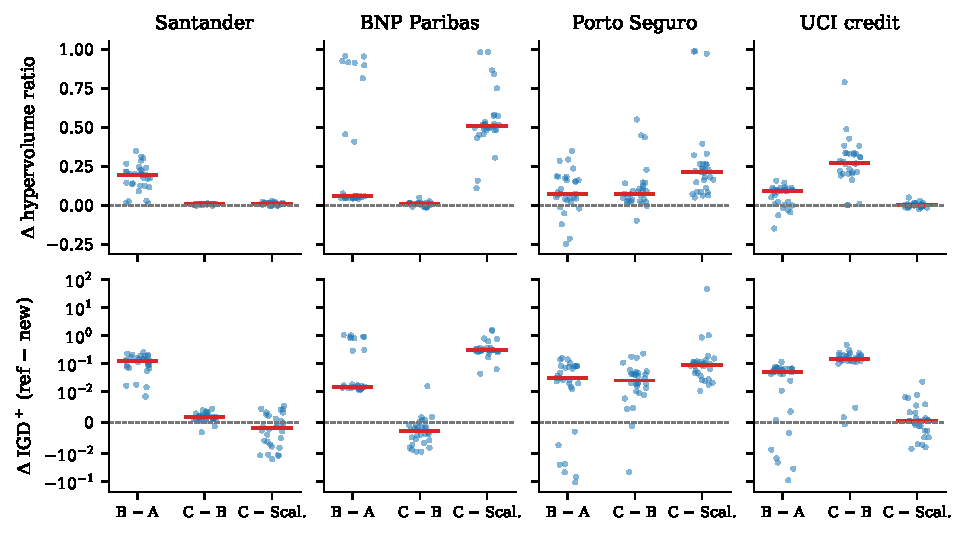
\includegraphics[width=\textwidth]{fig04_paired_deltas.pdf}
\caption{Paired differences on the two primary endpoints, one point per outer partition, red bar at the median; the
IGD$^+$ axis is symmetric-logarithmic. The BNP Paribas NBI-B $-$ NBI-A distribution is visibly bimodal: small positive
differences plus a tail of seven partitions where NBI-A collapses.}
\label{fig:paired}
\end{figure}

Three qualifications bound this. First, corrected significance is the exception here, not the rule. Of the sixteen
primary tests that carry the two NBI comparisons (two comparisons $\times$ two endpoints $\times$ four datasets,
weighted cost), five reach Holm-corrected $p < 0.05$: both Santander anchor tests, NBI-C versus NBI-B on Santander
hypervolume, and both UCI credit NBI-C tests (\cref{tab:paired}). The other eleven do not: every test on BNP
Paribas and Porto Seguro, both UCI credit anchor tests, and Santander $\igdp$ for NBI-C versus NBI-B. On BNP Paribas
the effect is unanimous in sign yet the corrected $p$ is $0.66$, because the differences are bimodal (the mean
$+0.279$ is over four times the median $+0.058$), so by the rule of \cref{sec:protocol:stats} we report the median with
its bootstrap interval $[+0.051, +0.070]$, the win fraction with its Wilson interval and the rank-biserial correlation
(supplementary Section~S5). Those three quantities describe how \emph{consistent} a difference is across the 30
partitions of a dataset; none of them corrects for the partition overlap of \cref{sec:protocol:stats}, which is what
the corrected test exists to handle, so they do not establish significance and are not offered in its place. Where the
corrected test does not reach $0.05$ we report the comparison as consistent in direction and not statistically
established. Second, the Porto Seguro and UCI credit win rates are driven by the twenty partitions added in the
extension (hypervolume $18/20$ and $19/20$ against $6/10$ and $5/10$ with one tie in the first ten; on UCI credit the
batch difference has an uncorrected Fisher $p = 0.009$, an exploratory comparison discussed in
\cref{sec:results:r30}): the effect is consistent in direction across the 30 partitions but not statistically
established, and the first ten partitions alone did not show it. Third, it depends on the cost definition: under the
support cost Santander is unchanged ($30/30$) and Porto Seguro stays positive on $\igdp$ ($29/30$), but BNP Paribas
weakens to $19$--$20/30$, all ten of its hypervolume losses falling in the partitions whose support-cost
normalization box is narrow (\cref{sec:results:cost}), and UCI credit \emph{reverses}, NBI-B being worse in
$26$--$27/30$ partitions (full support-cost repetition in supplementary Section~S5).

\paragraph{How much of this is the relocated geometry?} Because a vertex value of $\beta$ returns its anchor directly,
NBI-B's returned set \emph{contains} the three real single-objective optima, which are also points of the empirical
reference. Part of the gain is therefore the injection of those extreme solutions rather than the relocated CHIM. We
separate the two by rescoring NBI-A's own candidate set augmented with the same three anchors, changing nothing else
(\texttt{scripts/\allowbreak pco213\_\allowbreak anchor\_\allowbreak injection\_\allowbreak control.py}; per-partition
results in supplementary Section~S12). Injecting the anchors alone closes a median $80\%$ of the
A-to-B hypervolume gap on Santander, $90\%$ on BNP Paribas, $49\%$ on Porto Seguro and $1\%$ on UCI credit, medians
taken over the partitions in which that gap is positive (all 30 on the first two datasets, 24 on the other two). The
residual, which is the part attributable to the relocated geometry, has median $+0.038$, $+0.005$, $+0.021$ and
$+0.091$ hypervolume respectively over all 30 partitions.

This materially qualifies the headline. On Santander and BNP Paribas the mechanism is mostly the returned extreme
points, not the CHIM; on UCI credit it is almost entirely the CHIM; Porto Seguro is intermediate. The practical
recommendation is unchanged and if anything simpler: compute the real single-objective optima and make sure they
reach the returned set, whether by re-anchoring or by adding them. The causal story, however, must be stated at this
resolution rather than as ``relocating the CHIM repairs the front''.

\paragraph{What goes wrong when anchors come from the surrogate.} NBI-A's BNP Paribas hypervolume ratio collapses in
seven of thirty partitions, exactly those in which the parsimony rule selects the \emph{quadratic} ROC-AUC order
($7/7$ against $0/22$ of the linear-selected ones; the remaining partition selects the special cubic order). A quadratic surface moves the surrogate AUC anchor off the
gradient-boosting vertex to an interior mixture the empirical reference dominates; anchor cost tracks the collapse,
but one partition collapses with a cheap anchor, making cost a marker rather than the mechanism (per-partition ratios
and anchor costs in supplementary Section~S6).

The consequence for the gate is uncomfortable. Because the quadratic ROC-AUC order is selected precisely when it
predicts unseen points better, the collapsed partitions have \emph{higher} ROC-AUC external $\rext$ (median 0.46 against
0.08) and their ROC-AUC surface passes the gate \emph{more} often (3 of 7 against 2 of 23) than those where NBI-A works:
the ROC-AUC gate does not single out this failure, while real anchors remove it, NBI-B reaching $0.935$--$0.996$ in all
thirty partitions. It also settles how the gate-conditional analysis must be read: the apparently larger anchor
benefit where the ROC-AUC gate passes on BNP Paribas ($+0.64$ against $+0.21$) is NBI-A's collapse restated, since three
of the five gate-passing partitions are collapse partitions, and is not evidence that real anchors add more when the
ROC-AUC surface is reliable.

\begin{figure}[t]
\centering
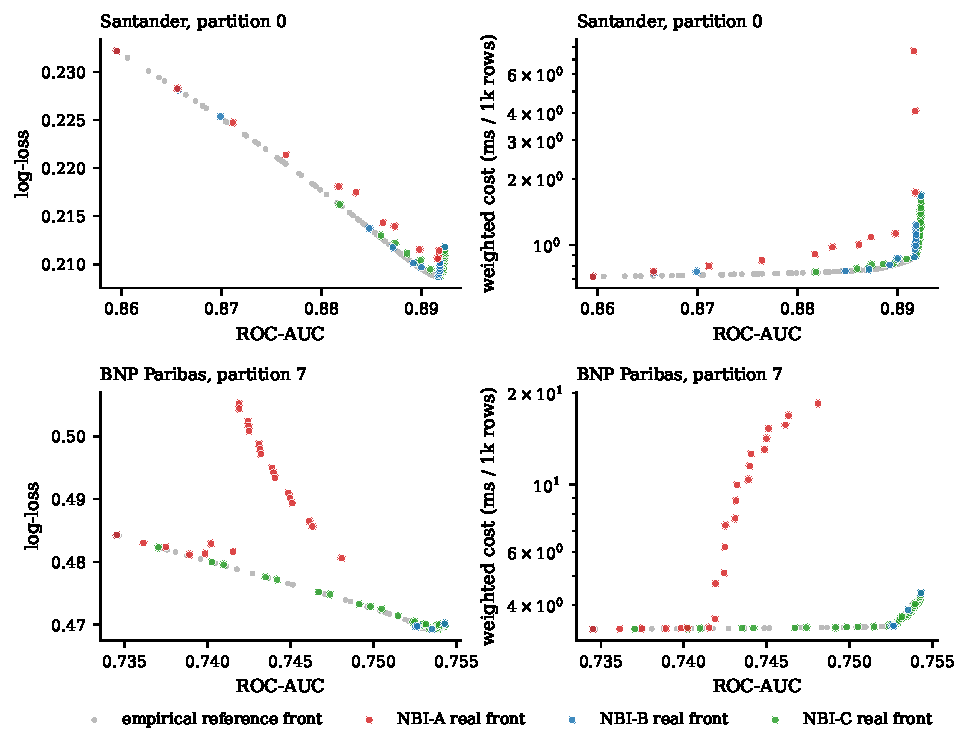
\includegraphics[width=\textwidth]{fig03_nbi_fronts.pdf}
\caption{Revalidated fronts of the three NBI variants against the empirical Pareto reference, in the
accuracy--calibration and accuracy--cost projections, for one Santander partition (top) and one BNP Paribas collapse
partition (bottom). Surrogate anchors displace the NBI-A front away from the reference and up the cost axis.}
\label{fig:fronts}
\end{figure}

\subsection{RQ5: Surrogate NBI against metamodel-free NBI}
\label{sec:results:metamodelfree}

NBI-C gives the best or tied-best approximation among the surrogate-derived methods on every dataset
(\cref{sec:results:nsga2} shows an external evolutionary optimizer does better still). NBI-C's median hypervolume
ratio is $0.989$, $0.983$, $0.982$ and $0.976$. It exceeds $0.95$ in all thirty partitions of three datasets and in
$26/30$ on Porto Seguro (worst partition $0.877$; per-partition counts in supplementary Section~S4). Against NBI-B it
wins on hypervolume in $28$, $24$, $28$ and $30$ of 30 partitions, at medians of $+0.0084$, $+0.0106$, $+0.074$ and
$+0.275$, the corrected test reaching significance on Santander ($p = 0.003$) and UCI credit ($p = 0.010$).

Set beside the anchor effect of \cref{sec:results:anchors}, these medians do not order the two steps the same way on
the four datasets. Removing the metamodel adds far less than moving the anchors on Santander and on BNP Paribas; on
Porto Seguro the two are a near-tie on the median and reverse on the mean; and on UCI credit the ordering reverses
outright, removal adding three times what the anchors add (supplementary Section~S5). Two clean datasets, one tie and
one reversal over four datasets is an observation about these problems, not a tested ordering, and it is weakened
further by the confound of \cref{sec:method:nbi}: NBI-C differs from NBI-B in the solver acceptance rule as well as in
the objective source, so the \emph{ratio} of the two effects is weaker evidence than either effect on its own.

Three caveats bound the NBI-C result. On BNP Paribas the two endpoints disagree, but the disagreement is a property of
the reference definition rather than of the arms. Against the augmented reference of \cref{tab:paired}, NBI-C covers
more volume ($24/30$, median $+0.0106$) while NBI-B is closer in $\igdp$ ($24/30$); against the sample core, which
contains no output of the compared methods, the $\igdp$ comparison reverses (NBI-C is closer in $20/30$) while the
hypervolume direction is
unchanged ($24/30$) (supplementary Section~S5). We therefore withdraw the earlier reading of this as a genuine
hypervolume/$\igdp$ trade-off between the arms and record it as reference-dependent. The large UCI credit gap is not a
surrogate-accuracy effect --- those surfaces pass the gate in every partition --- but a convergence effect of NBI-B,
which certifies a median of 29 of its 66 subproblems while indicators use converged candidates only; retaining its
unconverged iterates preserves the direction ($30/30$) but cuts the mean gap from $+0.277$ to $+0.108$ (supplementary
Section~S7). Neither observation supports a claim that interior surrogate error dominates once anchors are right.
Third, the premium is large and uneven (\cref{tab:compute}): NBI-C's solve records about $4.2\times10^{5}$ real
objective evaluations per replication, counting each ROC-AUC and each log-loss computation, whereas the surrogate
arms' solves record none. Charged standalone, so that each arm carries the stages it depends on, the premium of NBI-C
over NBI-B is $6.2$, $5.9$, $5.9$ and $2.3\times$: smallest on UCI credit, where it buys the largest gain, and largest on
Santander, where it buys $+0.008$ hypervolume. Among the NBI variants, metamodel-free NBI is not
uniformly preferable: what its premium buys depends strongly on the dataset.

\begin{table*}[t]
\centering
\caption{Standalone cost of each NBI variant: mean wall-clock seconds per partition (Apple M4 Max, 14 cores)
and mean real out-of-fold objective evaluations, charging every arm for everything it needs to run on its own
(design, gate and ROC-AUC-search entries count evaluated compositions; NBI-C's solve counts each ROC-AUC and each
log-loss computation, two per weight-vector evaluation).
NBI-A is charged the 66-run design, the 100 gate compositions and the Scheff\'e fit (``design\,+\,fit''), since its
anchors are the optima of the fitted surfaces; NBI-B is charged the same \emph{plus} the single-objective reference
stage, which is where its real anchors come from and which is dominated by the direct ROC-AUC search over
$4\times10^{4}$ sampled compositions; NBI-C is charged the reference stage and its own solve, and needs neither the
design nor the surfaces. Real anchors are therefore not free: NBI-B costs 1.2--12.7$\times$
the standalone wall clock of NBI-A, and the standalone premium of NBI-C over NBI-B is 6.2, 5.9, 5.9 and 2.3$\times$
(Santander, BNP Paribas, Porto Seguro, UCI credit), not the solver-stage ratio. Charging the whole reference stage to
NBI-B and NBI-C is an upper bound, since that stage also computes references the arms do not consume, and the SLSQP
log-loss anchor's evaluations are not separately instrumented. Not charged to any arm: the shared out-of-fold stage
(335, 86, 69, 11~s) and the study's own instrumentation, namely the empirical reference, quality scoring and
comparators (270, 154, 302, 74~s). ``Success'' is the mean fraction of the 66 subproblems that terminated
successfully (A/B: SLSQP-certified; C: equality-feasible under the lenient rule of \cref{sec:method:nbi}).
Source: \texttt{tables/stage\_times.csv}, \texttt{tables/nbi\_runs.csv}, \texttt{references.json} and
\texttt{design\_points.npz} of the frozen replications.}
\label{tab:compute}
\small
\setlength{\tabcolsep}{4pt}
\resizebox{\textwidth}{!}{%
\begin{tabular}{l l rrr r r r r}
\toprule
& & \multicolumn{3}{c}{Stage means (s)} & \multicolumn{2}{c}{Standalone} & Real & \\
\cmidrule(lr){3-5}\cmidrule(lr){6-7}
Dataset & Arm & Design\,+\,fit & Single-obj.\ refs & NBI solve & total (s) & vs.\ NBI-A & evals & Success \\
\midrule
\multirow{3}{*}{Santander} & NBI-A & 4.1 & --- & 34.0 & 38.1 & 1.0$\times$ & 166 & 0.98 \\
 & NBI-B & 4.1 & 444.5 & 34.6 & 483.1 & 12.7$\times$ & $4.1\times10^{4}$ & 0.95 \\
 & NBI-C & --- & 444.5 & 2528.4 & 2972.9 & 78.0$\times$ & $4.5\times10^{5}$ & 0.83 \\
\addlinespace
\multirow{3}{*}{BNP Paribas} & NBI-A & 2.2 & --- & 23.1 & 25.3 & 1.0$\times$ & 166 & 0.95 \\
 & NBI-B & 2.2 & 243.2 & 35.6 & 281.1 & 11.1$\times$ & $4.1\times10^{4}$ & 1.00 \\
 & NBI-C & --- & 243.2 & 1409.8 & 1653.0 & 65.2$\times$ & $4.6\times10^{5}$ & 0.83 \\
\addlinespace
\multirow{3}{*}{Porto Seguro} & NBI-A & 4.0 & --- & 84.8 & 88.8 & 1.0$\times$ & 166 & 0.58 \\
 & NBI-B & 4.0 & 441.2 & 55.8 & 501.0 & 5.6$\times$ & $4.1\times10^{4}$ & 1.00 \\
 & NBI-C & --- & 441.2 & 2504.5 & 2945.7 & 33.2$\times$ & $4.6\times10^{5}$ & 0.98 \\
\addlinespace
\multirow{3}{*}{UCI credit} & NBI-A & 0.5 & --- & 124.8 & 125.3 & 1.0$\times$ & 166 & 0.39 \\
 & NBI-B & 0.5 & 54.1 & 99.7 & 154.4 & 1.2$\times$ & $4.1\times10^{4}$ & 0.48 \\
 & NBI-C & --- & 54.1 & 306.6 & 360.7 & 2.9$\times$ & $4.7\times10^{5}$ & 0.98 \\
\bottomrule
\end{tabular}}
\end{table*}


\paragraph{Cheap comparators.} Random weighted scalarization is strong on UCI credit, whose surfaces pass the gate
in every partition, and on Santander, whose log-loss surface always passes it although its ROC-AUC surface never does;
it collapses on BNP Paribas, whose surfaces rarely pass (\cref{tab:gate}), to a median of one front point and
hypervolume ratio $0.474$. It ties NBI-C on UCI credit (differences within $\pm 0.002$, win fractions $16/30$ and
$18/30$, corrected $p = 1.00$). On Santander it trails NBI-C narrowly on hypervolume ($0.978$ against $0.989$; NBI-C
better in $25/30$, corrected $p = 0.06$) and beats it on $\igdp$ in $20/30$ (corrected $p = 0.35$), but both readings
depend on the reference: against the sample core, which contains no output of the compared methods, both move toward
NBI-C and the $\igdp$ majority reverses (computed from
\texttt{nsga2/\allowbreak nsga2\_\allowbreak pareto\_\allowbreak quality.csv}; supplementary Section~S5). The comparison is
confounded and we say so: NBI-C optimizes exact objectives while scalarization optimizes surrogates, so its BNP
Paribas and Porto Seguro advantage cannot be attributed to the NBI construction rather than to the objective source.
On identical surfaces NBI-B beats scalarization $30/30$ on BNP Paribas and $25/30$ on Porto Seguro but loses $29/30$
on UCI credit.

The 66-point random Dirichlet sample loses to NBI-C in every partition and to random scalarization in at least 28 of
30 on every dataset. It also loses to NBI-A and NBI-B in every partition except on UCI credit, where it beats NBI-A in
25 of 30 partitions on hypervolume and 24 on $\igdp$, and NBI-B in 14 and 17 respectively. The sample's hypervolume
ratio is exactly zero in up to $25/30$ partitions (supplementary Section~S4), because uniform compositions cost 8 to
20 times more than the reference front. The unoptimized 66-run mixture design also beats the sample $30/30$
everywhere. The sample is, however, matched to the NBI sets only in the number of candidates returned, so this is a
floor check and no efficiency claim is made from it.

One negative result bears on the classical motivation for NBI recalled in \cref{sec:method:nbi}: the even spread of
subproblems over the CHIM does not survive revalidation on the real objectives, under any spacing definition we
computed. NBI-C's size-matched spacing percentile is $0.99$, $0.54$, $0.96$ and $0.41$, against $1.00$, $1.00$, $1.00$
and $0.93$ for the random Dirichlet sample; \cref{sec:results:nsga2} shows this is a property of the construction, not
of the objective geometry.

\subsection{RQ5b: An external evolutionary baseline}
\label{sec:results:nsga2}

Everything above compares methods within one methodological family; the external question is whether a canonical
evolutionary optimizer, given the same objectives, behaves differently. We ran NSGA-II \citep{deb2002nsga2}
in pymoo \citep{blank2020pymoo} on exactly the three real out-of-fold objectives NBI-C optimizes, with a population of
66 matching the 66 NBI directions, library-default variation operators, a deterministic simplex repair, and a
termination budget set \emph{per replication} to NBI-C's recorded count of real objective evaluations there; the
configuration was fixed and committed before any run, so no operator setting was chosen by inspecting performance
(supplementary Section~S13). NSGA-II's evaluation counter, however, records weight-vector evaluations, each of which
computes both ROC-AUC and log-loss, whereas NBI-C's records each ROC-AUC and each log-loss computation separately, two
per weight-vector evaluation. The realized ratio of the two counts across the 120 replications, $0.999996$ overall and
within $[0.99992, 1.00010]$ per run, therefore means that NSGA-II performed twice as many weight-vector evaluations as
NBI-C's solve (about $1.7$ times as many if NBI-C is also charged its ROC-AUC anchor search). The comparison is matched
neither in weight-vector evaluations nor in time, and the wall-clock ratio is reported separately. Because the
empirical reference is augmented with candidate sets, adding a method changes it, box included
(\cref{sec:method:normbox}); we therefore score twice, against a \emph{sample-core} reference containing no output of
the five compared methods, and against a \emph{common augmented union} that includes NSGA-II and against which every
method's indicators are recomputed.

\begin{table*}[t]
\centering
\caption{NSGA-II against metamodel-free NBI (NBI-C), weighted cost, scored against the common augmented reference.
Both optimize the same three real out-of-fold objectives. NSGA-II's budget was set per replication to NBI-C's count of
real objective evaluations (realized ratio 0.999996 overall, 0.99992--1.00010 per run), but that count records ROC-AUC
and log-loss separately, so NSGA-II performed twice as many weight-vector evaluations. $\Delta$ is the
paired difference signed so that $\Delta > 0$ favours NSGA-II, with its percentile-bootstrap 95\% interval, the
win/tie/loss count over 30 partitions and the Holm-corrected Nadeau--Bengio $p$. The last column is the wall-clock
ratio, which is not matched either. The direction is the same under the sample-core reference, which contains no
output of the five compared methods: median $\Delta \mathrm{IGD}^+$ $+0.0047$, $+0.0075$, $+0.0065$ and $+0.0034$
(W/T/L $29/0/1$, $30/0/0$, $28/0/2$, $24/0/6$) and median $\Delta$ HV ratio $+0.0060$, $+0.0098$, $+0.0113$ and
$+0.0114$ ($30/0/0$, $30/0/0$, $26/0/4$, $30/0/0$), in row order, with the same cells reaching corrected significance.
Source: \texttt{reports/pco213\_postwork\_benchmark/nsga2/}.}
\label{tab:nsga2}
\small
\setlength{\tabcolsep}{4pt}
\resizebox{\textwidth}{!}{%
\begin{tabular}{l rr lcc lcc c}
\toprule
& \multicolumn{2}{c}{Median HV ratio} & \multicolumn{3}{c}{$\Delta \mathrm{IGD}^+$} & \multicolumn{3}{c}{$\Delta$ HV ratio} & Time \\
\cmidrule(lr){2-3}\cmidrule(lr){4-6}\cmidrule(lr){7-9}
Dataset & NBI-C & NSGA-II & median [95\% CI] & W/T/L & $p$ & median [95\% CI] & W/T/L & $p$ & ratio \\
\midrule
Santander & 0.990 & 0.998 & +0.0060 [+0.0039, +0.0074] & 29/0/1 & 0.026 & +0.0083 [+0.0063, +0.0110] & 30/0/0 & 0.026 & 2.2$\times$ \\
BNP Paribas & 0.981 & 0.994 & +0.0087 [+0.0078, +0.0094] & 30/0/0 & $<$0.001 & +0.0127 [+0.0113, +0.0139] & 30/0/0 & $<$0.001 & 2.2$\times$ \\
Porto Seguro & 0.981 & 0.995 & +0.0048 [+0.0035, +0.0075] & 26/0/4 & 0.577 & +0.0115 [+0.0070, +0.0169] & 26/0/4 & 0.577 & 2.2$\times$ \\
UCI credit & 0.977 & 0.988 & +0.0032 [+0.0011, +0.0045] & 23/2/5 & 0.131 & +0.0114 [+0.0071, +0.0156] & 30/0/0 & 0.023 & 2.3$\times$ \\
\bottomrule
\end{tabular}}
\end{table*}


The answer is unambiguous and we state it plainly: NSGA-II attains a better approximation than NBI-C on both
primary endpoints, on all four datasets, under both reference definitions (\cref{tab:nsga2}, whose caption gives the
sample-core repetition). All 16 dataset $\times$ endpoint $\times$ reference cells favour NSGA-II, with
rank-biserial correlations between $+0.87$ and $+1.00$. The corrected test reaches significance on Santander, BNP
Paribas and UCI credit hypervolume; on Porto Seguro the paired differences are heavy-tailed (mean $+0.021$ against
median $+0.011$), so by the rule fixed in advance the median, the win fraction and the effect size are the evidence
there, and all three agree.

Four qualifications matter. The margins are small in absolute terms: median hypervolume-ratio gains of $+0.006$ to
$+0.013$, on a scale where NBI-C already reaches $0.977$--$0.990$. The comparison is also not
cardinality-matched: NSGA-II returns exactly 66 mutually non-dominated points in all 120 runs, against NBI-C
revalidated front sizes whose medians are $35$, $34$, $56$ and $65$. Hypervolume is monotone under set inclusion and
$\igdp$ improves with additional points near the reference, so the larger returned set mechanically helps NSGA-II on
both endpoints, and within datasets the per-partition cardinality gap correlates with the hypervolume-ratio gap at
Pearson $+0.50$, $-0.37$, $+0.57$ and $+0.68$ against the common augmented union. Set size cannot explain the whole
margin on UCI credit, where the hypervolume gap is $+0.0114$ although the two sets differ by a median of one point,
but elsewhere it may explain part of it, so the reported margins should be read as an upper bound on NSGA-II's
advantage. NSGA-II used about $2.2\times$ the wall clock of NBI-C's solve: twice the weight-vector evaluations at a
similar time per evaluation. All NSGA-II runs except one pilot run were executed eight at a time as concurrent
processes (Reproducibility statement). And NSGA-II supplies 8--29\% of the augmented reference front (a mean over four probed
replications per dataset; supplementary Section~S8), so like NBI-B
and NBI-C it is partly graded against its own output there, which is why the sample-core reference, to which it
contributes nothing, is reported alongside; it gives the same answer.

This also settles what the surrogate-only comparison could not: whether NBI's lost spacing advantage reflects the
objective geometry or the CHIM construction. NSGA-II's crowding-distance selection produces markedly more evenly
spaced revalidated fronts on every dataset --- median spacing coefficient of variation $0.74$, $0.62$, $0.60$ and
$0.65$ against NBI-C's $2.28$, $0.88$, $1.56$ and $1.92$ --- so even spacing here is attainable and CHIM-based
construction does not deliver it. Scored post hoc under the support cost, which NSGA-II never optimized, the advantage
largely transfers (supplementary Section~S13), most strongly on BNP Paribas; the one reversal is Santander $\igdp$, where
NBI-C is marginally closer in 17 of 30 partitions.

This bounds one claim: NBI-C is best or tied-best \emph{among the surrogate-derived methods}, not among
multiobjective optimizers generally. It leaves untouched every conclusion about the surrogate pipeline itself
(reliability, anchor misplacement, the ROC-AUC gate's blind spot, the coefficient result, the cost-definition result),
because NSGA-II is not part of that pipeline and was never proposed as a component of it. A single untuned NSGA-II
configuration on the same objectives, given twice the weight-vector evaluations of NBI-C's solve, gave a modestly but
consistently better approximation on these four datasets, at about $2.2\times$ the wall clock. Whether NSGA-II also
leads at an equal number of weight-vector evaluations was not tested.

\subsection{RQ6: The actual multiobjective conflict}
\label{sec:results:conflict}

In objective space the conflict between discrimination and calibration is almost degenerate: the direct ROC-AUC
optimum exceeds the SLSQP log-loss optimum by $0.00068$, $0.00080$, $0.00006$ and $0.00034$ ROC-AUC --- 5 to 100 times
less than the gain from ensembling at all. Two qualifications prevent the stronger statement that the problems are the
same: the optima differ in weight space, the Porto Seguro pair practically coinciding (supplementary Section~S9), and
Santander pays $0.0032$ of log-loss for its $0.00068$ of ROC-AUC, so the practitioner gets a different \emph{model}
even where the objective values are nearly indistinguishable. An apparent $+254$~ms per 1{,}000 rows deployment-cost
gap on Santander did not survive checking and we do not claim it: it is an artifact of the activity threshold in
\cref{eq:supportcost} (supplementary Section~S9).

\subsection{RQ7: Effect of the cost definition}
\label{sec:results:cost}

\begin{figure}[t]
\centering
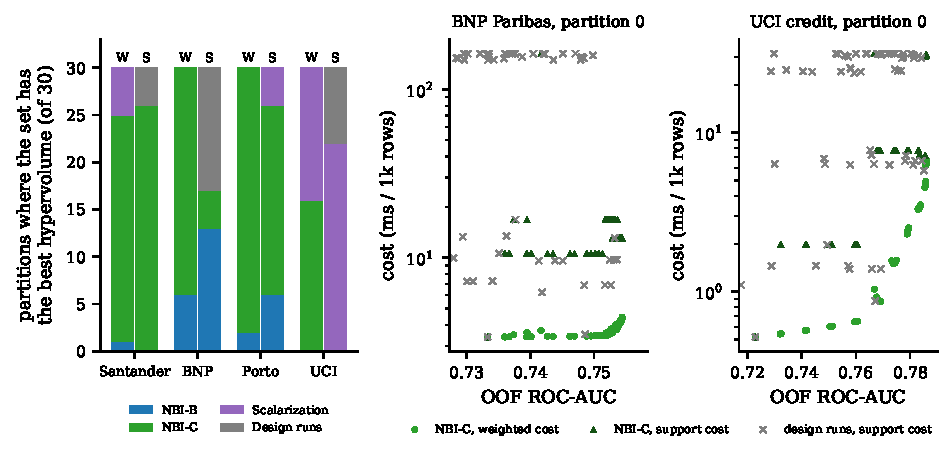
\includegraphics[width=\textwidth]{fig08_cost_definition.pdf}
\caption{Left: which method attains the best hypervolume, per dataset, under the weighted cost (W) and the support
cost (S), over 30 partitions. Right: one NBI-C candidate set scored under both definitions against the raw design
runs, for one BNP Paribas and one UCI credit partition. Under the step cost the design runs occupy cheap supports the
NBI sets, optimized on the linear relaxation, do not reach.}
\label{fig:cost}
\end{figure}

\begin{table}[t]
\centering
\caption{Holdout ranking agreement (partitions in which the OOF-best knee pick among NBI-A/B/C and scalarization is also holdout-best, weighted cost) and cost-definition sensitivity (partitions in which the hypervolume-best set differs between the weighted and the support cost; median Spearman correlation of the set rankings). Wilson 95\% intervals. Sources: \texttt{statistics/proportion\_intervals.csv}, \texttt{statistics/cost\_definition\_sensitivity\_r30.csv}.}
\label{tab:holdout_cost}
\small
\begin{tabular}{l l l r}
\toprule
Dataset & Holdout ranking agreement & Best set differs (W vs S) & Rank $\rho$ (W vs S) \\
\midrule
Santander & 30/30 [0.89, 1.00] & 10/30 [0.19, 0.51] & 0.83 \\
BNP Paribas & 15/30 [0.33, 0.67] & 24/30 [0.63, 0.90] & 0.89 \\
Porto Seguro & 23/30 [0.59, 0.88] & 8/30 [0.14, 0.44] & 0.94 \\
UCI credit & 30/30 [0.89, 1.00] & 20/30 [0.49, 0.81] & 0.66 \\
\bottomrule
\end{tabular}
\end{table}


The two cost definitions disagree often enough to change conclusions (\cref{fig:cost}, \cref{tab:holdout_cost}): the
hypervolume-best method changes between them in 8 to 24 of 30 partitions depending on the dataset (supplementary
Section~S9). NBI-C remains best under both on Santander and Porto Seguro ($26/30$ and $20/30$); on UCI credit random
scalarization takes the support-cost hypervolume in $22/30$, and several paired readings reverse outright
(\cref{sec:results:anchors}, \cref{sec:results:metamodelfree}).

The mechanism, where it can be isolated, is that a method optimizing $\sum_i w_i c_i$ has no incentive to zero out a
component. The raw 66-run design occupies exactly the cheap supports the NBI sets miss and can win outright under a
step cost when the normalization box's cost range excludes the $k$-nearest-neighbour region, as it does in the $13/30$
BNP Paribas partitions whose support-cost box is narrow (supplementary Section~S9).

One earlier reading did not survive scrutiny and we correct it here: the apparent bimodality of NBI-C's BNP Paribas
support hypervolume is a per-replication normalization artifact, not a regime --- the normalization box rescales the
cost axis tenfold between two groups of partitions, NBI-C's fronts are the same in both, and under a common bound the
split disappears (supplementary Section~S9). We therefore claim only the qualitative statement: NBI sets optimized on
the linear cost omit the cheapest supports the raw design contains, and the penalty's size depends on the chosen cost
range.

\subsection{RQ8: Transfer to the untouched holdout}
\label{sec:results:holdout}

In level, yes. The mean holdout-minus-out-of-fold ROC-AUC of every knee-selected solution lies within $\pm 0.005$ as a
point estimate, and the shift equals the weight-averaged shift of the base models on the same partition (correlation
$0.97$--$1.00$): a partition and refitting effect shared with the constituent models, not selection optimism.

In ranking, it depends on the dataset. The out-of-fold-best of the four knee picks is also holdout-best in $30/30$
partitions on Santander, $15/30$ on BNP Paribas, $23/30$ on Porto Seguro and $30/30$ on UCI credit, and the twenty
added partitions reproduce this pattern (supplementary Section~S10). The BNP Paribas figure measures how close the
four candidates are, not a failure of selection: their median out-of-fold gap is $0.0005$ against a holdout noise
standard deviation of about $0.0012$, and when the two disagree the holdout regret is at most $0.0022$ ROC-AUC. These
rates are specific to the selection rule and cost definition --- under the support cost they become $28$, $28$, $17$
and $16$ of 30 --- and are not dataset properties.

\subsection{RQ9: Did the first ten replications suffice?}
\label{sec:results:r30}

\begin{table*}[t]
\centering
\caption{Nested comparison of $R = 10$ with $R = 30$: mean hypervolume ratio and IGD$^+$ (weighted cost) of each NBI variant estimated from partitions 0--9 (the frozen $R = 10$ study, tag \texttt{pco213-postwork-r10}) and from all 30 partitions, with the $R = 30$ bootstrap interval and whether the $R = 10$ estimate lies inside it. Source: \texttt{statistics/r10\_vs\_r30\_stability.csv}.}
\label{tab:r10r30}
\small
\resizebox{\textwidth}{!}{%
\begin{tabular}{ll rll rll}
\toprule
& & \multicolumn{3}{c}{Hypervolume ratio} & \multicolumn{3}{c}{IGD$^+$} \\
\cmidrule(lr){3-5}\cmidrule(lr){6-8}
Dataset & Set & $R=10$ & $R=30$ [95\% CI] & inside & $R=10$ & $R=30$ [95\% CI] & inside \\
\midrule
Santander & NBI-A & 0.846 & 0.800 [0.767, 0.833] & no & 0.0954 & 0.1321 [0.1078, 0.1573] & no \\
 & NBI-B & 0.982 & 0.980 [0.977, 0.982] & yes & 0.0085 & 0.0121 [0.0101, 0.0142] & no \\
 & NBI-C & 0.991 & 0.987 [0.985, 0.990] & no & 0.0069 & 0.0105 [0.0084, 0.0127] & no \\
BNP Paribas & NBI-A & 0.717 & 0.695 [0.560, 0.819] & yes & 0.2212 & 0.2502 [0.1234, 0.3877] & yes \\
 & NBI-B & 0.966 & 0.974 [0.969, 0.978] & no & 0.0138 & 0.0114 [0.0096, 0.0132] & no \\
 & NBI-C & 0.982 & 0.982 [0.981, 0.984] & yes & 0.0143 & 0.0142 [0.0134, 0.0151] & yes \\
Porto Seguro & NBI-A & 0.803 & 0.781 [0.750, 0.812] & yes & 0.0751 & 0.0911 [0.0765, 0.1055] & no \\
 & NBI-B & 0.820 & 0.866 [0.810, 0.913] & yes & 0.0695 & 0.0531 [0.0351, 0.0746] & yes \\
 & NBI-C & 0.973 & 0.974 [0.964, 0.983] & yes & 0.0113 & 0.0111 [0.0075, 0.0155] & yes \\
UCI credit & NBI-A & 0.661 & 0.639 [0.589, 0.693] & yes & 0.1854 & 0.2043 [0.1724, 0.2340] & yes \\
 & NBI-B & 0.670 & 0.699 [0.643, 0.751] & yes & 0.1809 & 0.1681 [0.1383, 0.2008] & yes \\
 & NBI-C & 0.975 & 0.976 [0.974, 0.979] & yes & 0.0107 & 0.0099 [0.0089, 0.0110] & yes \\
\bottomrule
\end{tabular}}
\end{table*}


\begin{figure}[t]
\centering
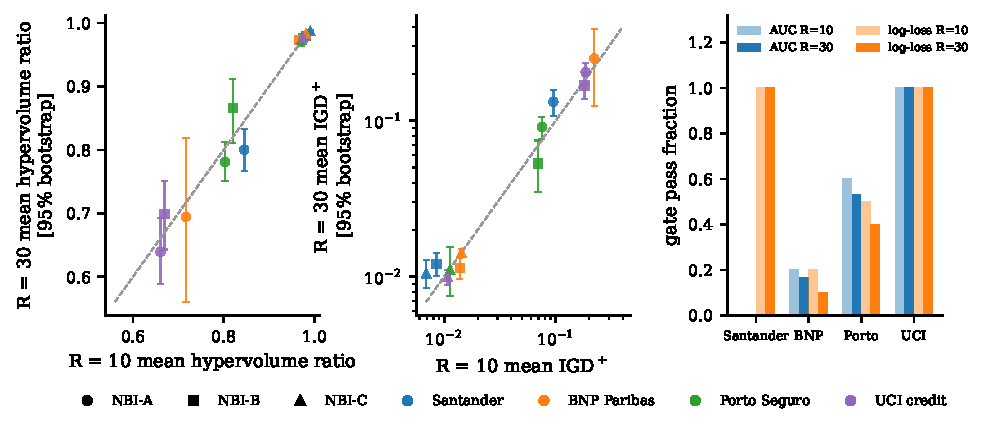
\includegraphics[width=\textwidth]{fig06_r10_vs_r30.pdf}
\caption{Mean indicator at $R = 10$ against $R = 30$ with bootstrap intervals (left, centre) and gate frequencies at
both sample sizes (right). Points on the diagonal are unchanged estimates.}
\label{fig:r10r30}
\end{figure}

Tripling the number of replications reversed no primary effect that is statistically established at $R = 30$, but it
did not leave every direction intact. Analysed separately, the first ten and the twenty new partitions give the same
sign of the median paired effect in 28 of the 32 primary cells, including all 13 that are statistically established
at $R = 30$, and the same four cells are the only ones whose sign differs between $R = 10$ and $R = 30$: the UCI
credit anchor effect on $\igdp$ (real anchors winning $5/10$ in the first ten partitions against $19/20$ in the new
ones), NBI-C versus random scalarization on Santander $\igdp$ (NBI-C winning $6/10$ against $4/20$), and NBI-C versus
random scalarization on UCI credit on both endpoints (medians within $\pm 0.0022$). The level comparison of
\cref{tab:r10r30} and \cref{fig:r10r30} is nested (partitions 0--9 are one third of the $R = 30$ sample), so its
agreement is partly built in: the $R = 10$ estimate lies inside the $R = 30$ bootstrap interval in 9 of 12
hypervolume cells, 7 of 12 $\igdp$ cells and all 8 gate frequencies, four of which are $0/30$ or $30/30$ and so cannot
fall outside. What the extension delivered is a change of status for three findings: the previously undecidable Porto
Seguro and UCI credit anchor effect; the BNP Paribas anchor collapse, now a quantified $7/30$ with an identified
trigger; and two cost readings shown to be artifacts, the BNP Paribas support-cost bimodality, which the ten-partition
analysis had noted but not resolved, and the Santander deployment-cost gap of \cref{sec:results:conflict}, which the
ten-partition report does not record (supplementary Section~S11). A fourth item on that list has since been
withdrawn: the NBI-C versus NBI-B hypervolume/$\igdp$ split on BNP Paribas is a property of the reference definition
and reverses under the sample core (\cref{sec:results:metamodelfree}), so the extension sharpened that estimate
without settling a finding.

The level check against the twenty new partitions alone is passed by only 6 of 12 hypervolume and 5 of 12 $\igdp$
cells; the shift is clearest on Santander, whose $\igdp$ is higher in the new partitions for all three NBI variants,
and the hypervolume anchor win rates are $6/10$ against $18/20$ on Porto Seguro (Fisher $p = 0.14$) and $5/10$ against
$19/20$ on UCI credit ($p = 0.009$), both uncorrected. The two batches were run on different days (partitions 0--9 on
4--6 September 2026, 10--29 on 6--8 September 2026; run conditions in \cref{sec:limitations}), and the difference between them
is unexplained. Except for the nested
comparison of \cref{tab:r10r30} and \cref{fig:r10r30}, which the statistical analysis plan specified, the comparisons
in this section are exploratory. The first ten partitions thus gave the direction of every established effect but not
every conclusion (supplementary Section~S11).
\section{Discussion}
\label{sec:discussion}

One claim organizes the results: on the classifier-weight simplex the mixture-design response surface is a good
\emph{description} of ensemble performance and an unreliable \emph{optimization substrate}, and the dominant error is
not inside the surface but in the points that build the geometry of the search.

\subsection{Why anchors dominate}
\label{sec:disc:anchors}

NBI derives its whole search geometry from the payoff matrix, so every subproblem in \cref{eq:nbi} is posed relative
to the individual optima. An anchor error is therefore global rather than local: it relocates the CHIM, redirects
every quasi-normal and rescales the objective space of all 66 subproblems, while an interior error of the same size
perturbs single solutions and leaves the frame intact.

The asymmetry predicts part of what we observe, but not all of the measured gap is geometry. Replacing surrogate
anchors with real ones, surfaces held fixed, improves both primary endpoints in $30/30$ partitions on the two datasets
whose ROC-AUC surfaces almost never pass the gate, and in $23$--$24/30$ on Porto Seguro and $24/30$ on UCI credit,
with hypervolume gains up to $+0.18$. That substitution changes four things at once (\cref{sec:method:nbi}), and one
of them is not geometric: because the three vertex values of $\beta$ return their anchor directly, NBI-B's candidate
set \emph{contains} the real single-objective optima, which are themselves points of the empirical reference. The
injection control of \cref{sec:results:anchors} separates that channel from the rest. Adding those same three points
to NBI-A's own candidate set, changing nothing else, already closes a median $80\%$ of the A-to-B hypervolume gap on
Santander and $90\%$ on BNP Paribas, against $49\%$ on Porto Seguro and $1\%$ on UCI credit. On Santander and BNP
Paribas --- the two datasets with the largest raw effect, and the first of them the only Holm-significant one --- most
of what the headline numbers measure is therefore the returned extreme solutions rather than the relocated CHIM. The
relocated-CHIM effect is cleanest on UCI credit, where it accounts for essentially the whole $+0.097$ hypervolume
residual; it is present but small elsewhere, positive in $30/30$ Santander and BNP Paribas partitions at a median
$+0.038$ and $+0.005$. The mechanism therefore survives at a smaller size than the raw contrast suggests, and the
practical recommendation is if anything simpler: compute the real single-objective optima and make sure they reach the
returned set, whether by re-anchoring or by adding them.

How much the surrogate still costs once the anchors are right is dataset-dependent, and no single ordering covers the
four: removing the metamodel entirely adds far less than real anchors did on two datasets, the same on a third and
three times as much on the fourth --- and on that third dataset the median and the mean disagree
(\cref{sec:results:metamodelfree}; supplementary Section~S5). Two clean cases, one
tie and one reversal over four datasets make that an observation rather than a tested claim, and because B versus C also changes the solver acceptance rule
(\cref{sec:method:nbi}), the \emph{ratio} of the two effects is weaker evidence than either effect on its own.

BNP Paribas shows how the anchors go wrong in the first place: where the parsimony rule selects a quadratic ROC-AUC
surface, the surrogate maximum sits at an interior mixture instead of the gradient-boosting vertex, so the CHIM is
built from a false utopia point and the front collapses (\cref{sec:results:anchors}) --- a geometric failure, not a
numerical one, since the solver certifies these subproblems, and invisible to any diagnostic computed on the surface
alone.

\subsection{Why the reliability gate does not catch it}
\label{sec:disc:gate}

The gate asks whether a surface predicts unseen compositions well on average; anchor placement depends on where the
surface puts its \emph{argmax}, a far more local property. A surface can be globally accurate and still misplace an
extremum, or globally poor with its argmax on the right vertex.

On BNP Paribas they diverge actively: the parsimony rule selects the quadratic order precisely when it predicts
held-out points better, so the collapse partitions have higher external $R^2$ and pass the gate more often than the
partitions where the surrogate anchor is right. A linear Scheff\'e surface has its maximum at a vertex by
construction, so the \emph{less} flexible model is accidentally protected while the more flexible one may place an
interior maximum the data do not support.

Hence a division of labour: the gate is worth its 100 extra evaluations for separating unusable surfaces from
excellent ones, but only the anchor check that distinguishes NBI-B from NBI-A removes the failure instead of
diagnosing it.

\subsection{Smooth surrogates against a rank statistic}
\label{sec:disc:smooth}

Two of the three objectives behave as the framework's engineering origins assume: log-loss is convex and smooth in
$\wvec$, and the Brier score is exactly quadratic in $\wvec$, so its surface reproduces it at $\rext = 1.000$ in all
120 replications --- an algebraic identity that checks the fitting code, not evidence about adequacy. The ROC-AUC is
not: a rank statistic, constant wherever the induced ordering does not change and kinked between orderings, which a
low-order polynomial smooths across instead of representing. Hence the Santander ROC-AUC surface reaches a Spearman
correlation of $0.830$ with a negative external $R^2$ --- ordering broadly right, values wrong.

The resulting bias is one-directional (\cref{sec:results:coefficients}): a quadratic fitted over an edge with one weak
endpoint absorbs that curvature into $\beta_{ij}$ and overshoots its maximum --- the same over-prediction of interior
optima that displaces surrogate anchors off vertices. Where the objective \emph{is} smooth in the weights the
machinery can work as advertised: Santander's log-loss surface passes the gate in every partition.

Non-smoothness is a contributing factor, not the explanation. Were it the explanation, the smooth convex objective
would be the reliable one everywhere, and it is not: log-loss surfaces pass the gate in $30/30$ partitions on
Santander and UCI credit but in only $3/30$ on BNP Paribas and $12/30$ on Porto Seguro. On BNP Paribas the smooth
objective does no better than the rank statistic ($3/30$ against $5/30$ at the pre-specified gate thresholds and the
component clip of \cref{sec:protocol:models}; median $\rext$ of $-0.180$ against $+0.118$); on Porto Seguro the two
are effectively tied ($12$ against $16$). Only Santander
shows the sharp separation the smoothness account predicts ($\rext$ $0.971$ for log-loss against $-0.333$ for
ROC-AUC), and one dataset is an illustration rather than a mechanism. What these data establish is that adequacy
varies by dataset \emph{and} by metric and has to be measured on unseen compositions; they do not identify what,
besides the shape of the response in $\wvec$, makes a given dataset--metric pair fittable by a low-order polynomial.

\subsection{Non-smoothness also constrains the optimizer}
\label{sec:disc:solver}

The same property constrains the metamodel-free arm: SLSQP cannot certify optimality on a piecewise-constant
objective, whose gradient is zero almost everywhere, so NBI-C accepts a feasible iterate under the weaker rule of
\cref{sec:method:nbi}, not the certification NBI-A and NBI-B obtain on smooth polynomials. Success rates are
therefore not on a common scale across arms, and we do not read the difference as evidence about surrogate quality.

UCI credit shows why that care is needed: its $+0.277$ hypervolume gain for NBI-C over NBI-B, at Holm-corrected
$p = 0.010$, looks like the strongest evidence here for the metamodel-free arm, yet UCI credit's surfaces pass the
gate in every partition, so surrogate error cannot explain it: the gap tracks how many of NBI-B's 66 subproblems
certify, at Spearman $-0.92$, and disappears in the partitions where NBI-B converges fully (supplementary
Section~S7).

\subsection{Compute against fidelity}
\label{sec:disc:compute}

Among the surrogate-derived methods, metamodel-free NBI is best or tied-best on the primary endpoints, although an
external evolutionary optimizer on the same real objectives, given about twice NBI-C's weight-vector evaluations,
does better still (\cref{sec:results:nsga2}). Evaluating the real objectives throughout its solve, NBI-C costs 2.3 to
6.2 times the standalone wall clock of NBI-B (\cref{tab:compute}), and what that premium buys is strongly conditional:
on UCI credit the smallest premium buys the largest gain, while on Santander the largest buys $+0.008$ hypervolume.

Its affordability is specific to this problem: one evaluation is a matrix--vector product plus a sort, $0.37$ to
$2.13$~ms here. Where each evaluation needs a model refit the ordering reverses and the surrogate is the only viable
route --- the regime the framework was designed for. The recommendation is therefore conditional on evaluation cost:
cheap evaluations should be used directly, at least for the anchors; expensive ones argue for an externally validated
surrogate, anchored on whatever real evaluations are affordable.

\subsection{Response surfaces as descriptions rather than optimizers}
\label{sec:disc:description}

The surfaces themselves are reproducible across resampled partitions (\cref{sec:results:coefficients}), and as a
description of which vertices are weak and which regions flat the model is interpretable in a way a black-box
optimizer is not. What does not survive is the step from that description to inference about blends: the classical
synergism criterion $\beta_{ij} > |\beta_i - \beta_j|$ is correct as stated and guards against reading the sign of
$\beta_{ij}$ alone, but it is computed \emph{from the surface}, so on these ensembles it inherits the surface's
systematic over-prediction of interior optima, and a candidate pair must be confirmed on the real objective --- one
matrix product.

\subsection{Deployment cost is not the cost that was optimized}
\label{sec:disc:cost}

Every method here minimized the continuous relaxation $\sum_i w_i c_i$, since a step cost is not differentiable and
cannot enter a gradient-based formulation; deployment pays the step cost. The two are not monotonically related inside
the simplex, and the consequence is not cosmetic: which of the six candidate sets attains the best hypervolume changes
between the definitions in 8 to 24 of the 30 partitions (\cref{sec:results:cost}; supplementary Section~S9), and
several paired conclusions reverse, including the anchor effect on UCI credit.

The mechanism is that a linear cost gives no incentive to zero a component: a weight of $0.01$ on a model costing
$200$~ms adds $2$~ms under the relaxation and $200$~ms in deployment. Methods optimizing the relaxation drift into the
interior and miss the cheap low-support solutions --- pure vertices and two-model faces --- that the unoptimized
66-run design contains by construction.

Whether a relaxation and the support it induces agree has been examined in one related setting, and the answer went
the other way: for budgeted learning with feature re-use, a support-cost programme is solved exactly by its linear
relaxation \citep{nan2016pruning}, a guarantee our setting does not inherit. Report which cost model is used; zero
weights below the activity threshold and re-evaluate, since an inert weight just above $\varepsilon$ produced a
spurious difference of about $250$~ms per 1{,}000 rows in our own analysis; and optimize over supports explicitly
where deployment cost is the
real objective.

\subsection{What the framework's transfer teaches}
\label{sec:disc:transfer}

The pipeline transfers where the response is smooth in the mixture components, a condition identifiable in advance.
Where the ROC-AUC surface is adequate too --- UCI credit, which passes in $30/30$ --- the cheap route is competitive:
random scalarization on those externally validated surfaces is statistically indistinguishable from the
metamodel-free arm (mean $\Delta\hv = +0.0015$ with bootstrap interval $[-0.003, 0.007]$, better in $16/30$;
indicator levels in supplementary Section~S4). Surrogate-assisted NBI with real anchors is not, but that
residual gap is a subproblem-convergence effect of NBI-B rather than surrogate error
(\cref{sec:disc:solver}). The stronger reason to stop early there is that there is very little to win: the gain of the
log-loss optimum over the best single model is an order of magnitude smaller than on the other three datasets, out of
fold and on the untouched holdout alike, and not separable from zero by a corrected test (supplementary
Section~S10). What UCI credit therefore shows is not that the inherited machinery is efficient but that on that
dataset \emph{no} weighting method separates from the best single model on held-out data, so the cheapest adequate
one suffices. The pipeline does not
transfer unexamined to a rank-statistic response, to anchors that are vertices of the feasible region rather than
interior points, or to an objective that is a step function of the support.

One connection this study does not establish is between front quality and the decision taken from the front.
\emph{Within} a candidate set, out-of-fold selection transfers to the holdout in level, and the out-of-fold-best of
the four knee picks is also holdout-best in $30/30$, $15/30$, $23/30$ and $30/30$ partitions
(\cref{sec:results:holdout}); across methods it is much weaker. Paired by partition under the weighted cost, the two
NBI contrasts that are Holm-significant on both primary endpoints have \emph{worse} single-objective holdout accuracy at
the knee-selected point, on ROC-AUC and on log-loss alike, and cheaper selected points (supplementary Section~S10).
These are different points of the same trade-off rather than a contradiction of indicator results computed over whole
fronts. They do not support the converse either: on these four datasets a better approximation of the front does not
reliably buy a better selected solution, and the two contrasts where the pick does improve are the ones with the
smaller indicator effects. Any statement that out-of-fold selection transfers must therefore be read as within-method
and in level, not as evidence that better fronts give better picks.

What we would carry forward is not a method but a checklist: external validation on unseen compositions, an argmax
check against the real optimum, revalidation on the true objective before scoring, a reference whose sampled core is
constructed independently of the surrogate and of every candidate method, and an explicit statement of which cost is
paid. Each of them changed a conclusion that would otherwise have been reported.

\section{Limitations}
\label{sec:limitations}

\paragraph{Four datasets is the binding constraint.} The statistical unit is one outer partition, but the unit of
\emph{generalization} is the dataset, and there are four. Every replication-level interval here describes partition
sensitivity within a dataset, not uncertainty about a population of datasets, so every cross-dataset mechanism
statement is an association over four points and not a tested hypothesis; in particular, the benefit of real anchors
does not track surrogate reliability (\cref{sec:results:anchors}). All four datasets are binary tabular problems of
$3\times10^{4}$ to $2\times10^{5}$ rows from financial-services applications, three of them from Kaggle competitions,
so the four points are not four independent domains. Nothing here establishes behaviour outside financial services,
on multiclass problems, text or image data, very small samples or ensembles of more than five members, where the
simplex and design grow quickly, and every conclusion is scoped to the one-shot, no-infill case
(\cref{sec:rel:surrogate}). Repeating the unchanged protocol on a broader, prospectively specified panel that includes
other domains is a natural next step.

\paragraph{The partitions ran in two batches.} Partitions 0--9 and 10--29 ran as two separate batches with the same recorded
platform and core count, and some indicator levels and anchor win rates differ between them (\cref{sec:results:r30}). A bounded
check of the existing records (supplementary Section~S11) found no recorded difference between the batches that could produce it, other than the pre-fix
stages of partition 0 inside the first (supplementary Section~S1): the
library source code was the same for partitions 1--29, the recorded package versions, platform and core count were
the same, seeds follow one rule, and the configuration differs only in the replication count and two bookkeeping
flags. No partition was computed in both batches, so determinism across the batches cannot be tested directly; the
one recomputation available, of the NBI stage of UCI credit partition 0, reproduced its stored candidates exactly.
The records do not include whether the working tree was clean, the linear-algebra backend, thread-related
environment variables, or the machine's power, thermal state and concurrent load, so we report the difference as
exploratory and cannot explain it; execution date alone is not an explanation. Every interval and test here treats
the 30 partitions of a dataset as exchangeable.

\paragraph{The gate is not an independent test.} The 100 external compositions of a partition both select the
Scheff\'e order and judge it (\cref{sec:method:scheffe}), so a gate pass is an optimistic reading of out-of-design
adequacy. A post hoc split-sample reading of the stored compositions (supplementary Section~S6) leaves the extreme
verdicts unchanged and, against selecting and judging on the same half, lowers intermediate pass counts; no evaluation set independent of order selection was
available, so the gate's decision utility is not established here.

\paragraph{Neither NBI contrast is a single-factor experiment.} Replacing the anchors changes four things at once
(\cref{sec:method:nbi}). The injection control of \cref{sec:results:anchors} separates the injected extreme points from
the other three, but no control in this study separates the utopia point, the normalization and the direction set from
one another; that would require an NBI implementation in which each can be varied independently. NBI-B versus NBI-C
also changes the solver acceptance rule, because certified optimality is generically unattainable on a
piecewise-constant ROC-AUC, so success rates are not on a common scale across arms, and the UCI credit gap between
NBI-C and NBI-B is substantially a convergence artifact of NBI-B (\cref{sec:results:metamodelfree,sec:disc:solver}).

\paragraph{The model zoo is fixed and shapes the findings.} Base learners and hyperparameters were fixed in advance
with no search: the study measures the weighting layer with the model layer held constant, so every empirical result
here is conditional on this zoo. The zoo contains a member that is poorly calibrated on three of the four datasets and
an expensive one ($k$-nearest neighbours alone costs more than the other four combined in every replication;
\cref{sec:protocol:models}), which makes the cost objective non-trivial and also drives the $\beta_{ij}$ result of
\cref{sec:results:coefficients}: the largest interactions attach to the weakest vertex. Whether the surface, anchor,
cost and coefficient results hold for a zoo of near-equal members is untested and left to future work.

\paragraph{The Pareto reference is empirical.} With no analytical front, all convergence and coverage indicators are
computed against a sample-based reference of about $10^{5}$ points per replication. Its weighted-cost front met the
5\% displacement tolerance in 118 of 120 replications and ended at most 6\% displaced in the other two
(supplementary Section~S8). The benchmark's check did not cover the support-cost front; a post hoc check from the
stored samples found that front less converged, meeting the tolerance in 6 to 12 of 30 replications per dataset
against 9 to 27 for the weighted-cost front under the same definition, so conclusions under the support cost also
carry reference instability. The final reference also
contains every candidate set, so methods contributing many points are partly graded against their own output. Those
points lower every arm's hypervolume ratio rather than inflating it, and can change a hypervolume contrast only
through the normalization box (\cref{sec:method:normbox}); under $\igdp$ they can favour their own arm. Against the
sample core no NBI-B versus NBI-A direction changes, but two small $\igdp$ readings reverse: NBI-C versus NBI-B on
BNP Paribas and NBI-C versus random scalarization on Santander (\cref{sec:results:metamodelfree}).

\paragraph{No comparison is compute-matched.} The arms are compared as specified, not at equal budget, so the
comparison supports no efficiency claim (\cref{tab:compute}). The only external baseline, NSGA-II
(\cref{sec:results:nsga2}), is one canonical algorithm in one untuned configuration, and nothing here ranks it against
MOEA/D, NSGA-III or a surrogate-assisted evolutionary method. Its budget was set from NBI-C's evaluation counter,
which records the ROC-AUC and the log-loss computation of each weight vector separately while NSGA-II's counts weight
vectors, so NSGA-II evaluated about twice as many weight vectors as NBI-C's solve; it also used about $2.2\times$ the
wall clock of that solve, with its runs executed eight at a time, and returned 66 non-dominated points against NBI-C
medians of 34 to 65, so its margins should be read as an upper bound on its advantage. It outperformed the metamodel-free arm on every dataset. Whether
NSGA-II also leads at an equal number of weight-vector evaluations was not tested. The low-budget question, what an
evolutionary method or a random-search ladder achieves on the 66 design points and 100 gate points the surrogate arms
use, is the one a surrogate paper most needs and the one we do not answer.

\paragraph{The cost objective is a measured proxy.} All $c_i$ are wall-clock medians on one workstation with a fixed
library stack, one thread configuration and a per-dataset batch size; both cost models ignore memory, model loading,
shared preprocessing and parallel execution of the members, and the $c_i$ would change with hardware, thread
allocation, batching, a compiled inference runtime, or an approximate-nearest-neighbour index replacing brute-force
search, which would remove the study's largest cost asymmetry. The support cost adds the threshold
$\varepsilon = 10^{-3}$ of \cref{eq:supportcost}, fixed before the study and never changed: an AUC-inert
$k$-nearest-neighbour weight just above it produced a spurious difference of about $250$~ms per 1{,}000 rows
(\cref{sec:results:conflict}), so any support cost needs a weight-cleaning step. Conclusions that depend on the
support cost are sensitive to $\varepsilon$ and to the cost range that sets the normalization box, and are
conditional on the active members running one after another (\cref{sec:method:cost}). The cost objective is realistic
for the setting measured, not universal.

\paragraph{No claim of universal dominance, and confounded comparators.} Among the surrogate-derived methods, NBI-C is
best or tied-best on the primary endpoints under the weighted cost on these four datasets; it ties with random
scalarization on UCI credit, is not statistically separated from it on Santander $\igdp$, where the direction depends
on the reference (\cref{sec:results:metamodelfree}), and loses its support-cost advantage on BNP Paribas and UCI
credit. Its advantage over scalarization on BNP Paribas and Porto Seguro is confounded with the objective source:
NBI-C optimizes exact objectives, scalarization optimizes surrogates, and separating the two would require a
scalarization arm on the cached out-of-fold objectives, which we did not run.

\paragraph{Selection rules and the holdout analysis.} Holdout transfer is verified only within a candidate set and in
level, for a knee rule under the weighted cost with TOPSIS and the support cost as sensitivity analyses
(\cref{sec:results:holdout}). Whether the arm with the better front also yields the better selected solution is
answered only descriptively, and in the negative at the selected point on the two NBI contrasts that are
Holm-significant on both primary endpoints (\cref{sec:disc:transfer}).

\section{Conclusion}
\label{sec:conclusion}

We transferred an established DoE--RSM--NBI framework from multiobjective engineering optimization and forecasting to
the design of weighted classifier ensembles under a measured deployment cost, and asked when its Pareto front can be
believed. Three NBI arms, defined by the source of the objectives and the source of the anchors, were compared over
four public binary tabular datasets $\times$ 30 partitions, with every candidate revalidated on the true out-of-fold
objectives and scored against an empirical reference. The main findings, each limited to one-shot pipelines without
infill, one fixed zoo of five classifiers and four datasets from one application domain, are the following.
\begin{itemize}
\item Surrogate adequacy depends on the dataset and the metric and must be measured on unseen compositions. ROC-AUC
surfaces passed the external reliability gate in 0, 5, 16 and 30 of 30 partitions on Santander, BNP Paribas, Porto
Seguro and UCI credit, and log-loss surfaces in 30, 3, 12 and 30; smoothness of the response in the weights does not
explain the difference on its own.
\item On Santander and BNP Paribas, anchor misplacement had the largest observed effect among failures attributable to
the surrogate pipeline. Under the continuous cost the arms optimize, real anchors improved both primary endpoints in
all 30 partitions of these two datasets, in 23 to 24 of 30 on Porto Seguro and in 24 of 30 on UCI credit, although
the improvement is significant after the Nadeau--Bengio correction and Holm adjustment only on Santander. On
Santander and BNP Paribas most of the hypervolume gain comes from returning the real single-objective optima rather
than from the relocated construction, and removing the metamodel once the anchors are right adds far less than the
anchors there, about as much on Porto Seguro and three times as much on UCI credit, where a subproblem-convergence
effect of the real-anchored surrogate arm (NBI-B) rather than surrogate error dominates; this ordering is an
observation, not a tested claim.
\item The gate screens surface accuracy, not anchor placement. On BNP Paribas, surrogate-anchored NBI (NBI-A)
collapses in exactly the seven partitions where the parsimony rule selects a quadratic ROC-AUC surface, which it does
when that surface fits unseen compositions better, and these partitions pass the ROC-AUC gate more often than the rest
(3 of 7 against 2 of 23); the gate therefore needs an accompanying anchor check.
\item The classical synergism criterion $\beta_{ij} > |\beta_i - \beta_j|$ holds for the leading classifier pair in
every partition of all four datasets, yet the real 50/50 blend beats its better member on only one of them, so a large
interaction coefficient must be confirmed on the real objective before it is read as complementarity.
\item The continuous cost the methods optimize and the step cost deployment pays disagree about the hypervolume-best of
six candidate sets in 8 to 24 of 30 partitions, and several paired conclusions, including the UCI credit anchor
effect, reverse between them. Sets optimized on the linear relaxation omit the cheapest supports that the unoptimized
design contains, at a penalty whose size depends on the cost range that sets the normalization box.
\item On the same three real objectives, NSGA-II approximated the front better than metamodel-free NBI (NBI-C) in all
eight dataset--endpoint comparisons, five of them significant after correction, and gave more evenly spaced
revalidated fronts. It used about twice NBI-C's weight-vector evaluations and about 2.2 times its wall clock (NSGA-II
runs executed eight at a time), and whether it also leads at an equal number of weight-vector evaluations was not
tested. Its returned sets are larger, which mechanically favours it on both endpoints, so its small margins should be
read as an upper bound on its advantage. This is one untuned configuration on four datasets from one domain, not a
general recommendation; it bounds what the NBI pipeline is worth, not the diagnosis of when it can be trusted.
\end{itemize}

What we carry forward is therefore a set of controls rather than a method: validate the surface on compositions it
has not seen; compare each surrogate-derived anchor with the optimum computed directly on the out-of-fold objective
and make sure the latter reaches the returned set; revalidate every candidate on the out-of-fold objectives before
scoring; build a reference whose sampled core contains no output of the compared methods; and state which cost is
being paid. Each changed a conclusion that would otherwise have been reported, and the anchor check is not free
(\cref{tab:compute}). The response surfaces remain a reproducible description of the ensemble-weight simplex: their
four largest interaction coefficients keep their sign across all thirty resamplings, the coefficient of variation of
the largest one lies between 0.007 and 0.17 across the eight dataset--metric surfaces, and they say something
interpretable about which components are weak. Reproducibility is not accuracy, however, and their fitted values
deserve trust only where a surface has been validated on compositions it has not seen; whether they are also a sound
optimization substrate must be checked on each problem with these controls. Replication mattered: the first ten
partitions gave the direction of every primary effect that is statistically established at $R = 30$, but left the
Porto Seguro and UCI credit anchor effect undecided ($6/10$ and $5/10$ on hypervolume), which only thirty partitions
showed to be consistent in direction.

\section*{Reproducibility statement}
\label{sec:repro}

\paragraph{Code and frozen states.} Code, manifests, aggregated tables, statistics and figures are in the repository
\texttt{caioribeiro99/doe\_nbi\_hpo\_project}. Two annotated tags freeze the study: \texttt{pco213-\allowbreak postwork-\allowbreak r10}
the ten-replication analysis and \texttt{pco213-\allowbreak postwork-\allowbreak r30} (commit \texttt{b3ed050}) the
thirty-replication analysis reported here (\cref{sec:results:r30} compares the two tags). The manuscript, figures and
tables are on the branch \texttt{paper/\allowbreak surrogate-\allowbreak nbi-\allowbreak ensemble-\allowbreak weighting}, cut from that tag, together with the results computed after it from the stored outputs of the
thirty-replication run, among them the NSGA-II baseline, the anchor-injection control and the blend test of
\cref{tab:edge}. A single checkpointed ten-stage runner drives the benchmark and
resumes an interrupted run without recomputation; its stages, the resumption planner, the aggregation and statistics
scripts and the coverage of the library's 83 unit tests are in supplementary Section~S1. The commit history records
that the library, the benchmark runner and the analysis and asset-building scripts were developed with the assistance
of Anthropic's Claude models (Claude Fable 5, Claude Fable 5.1 and Claude Opus 5) used through Claude Code; the
library's behaviour is checked by those unit tests.

\paragraph{Determinism and environment.} Every stochastic component is seeded as $\text{20260904} + r$ for
replication $r$; the offsets, the seed map, the configuration history and the resolved library versions are in the
master manifest (supplementary Section~S1). The environment is Python 3.11.15 with NumPy 2.4.6 \citep{harris2020numpy}, pandas 3.0.5,
SciPy 1.17.1 \citep{virtanen2020scipy}, scikit-learn 1.9.0 \citep{pedregosa2011scikit}, statsmodels 0.15.0 and
XGBoost 3.2.0 \citep{chen2016xgboost}, on macOS (Apple M4 Max, arm64), with eight worker threads. Execution provenance --- stage time and the fit, design, subproblem and objective-evaluation counts --- is in
supplementary Section~S1. Two stages were retried, both in the first ten replications; none in the extension.

\paragraph{Data availability and redistribution limits.} The raw datasets are not redistributed: the UCI
default-of-credit-card-clients data are downloadable from the UCI Machine Learning Repository, while the three Kaggle
datasets are subject to competition rules and must be obtained from Kaggle by the user. Per-dataset manifests record
the provenance (source, acquisition command, expected invariants and the SHA-256 checksum of the file actually
used), so a copy of the same file can be verified byte-for-byte (supplementary Section~S1). All three Kaggle training
files were obtained from public mirror datasets hosted on Kaggle and validated against those invariants; the
manifests name each mirror. Competition test labels are never used. Porto Seguro was subsampled to 200{,}000 rows
by a stratified draw with the recorded seed. The per-replication raw artifacts total about 829~MB and are
deliberately not version-controlled, but are reconstructible from the seeds and the runner, except for the
wall-clock costs $c_i$, which are re-measured on each run, and the results that depend on them; the measured costs
are committed in \texttt{tables/inference\_costs.csv}.

\paragraph{What a replication requires.} Reproducing the aggregate results from the published tables and statistics
requires only the repository; from raw data it requires the four datasets, the pinned environment and approximately 81
hours of single-workstation compute, or proportionally less for a subset of datasets or replications, since the
runner is resumable and parameterized by dataset and replication count.


\ifanon{\noindent Funding and acknowledgements are given on the separate title page.}{%
\section*{Funding}
This work was supported by the Funda\c{c}\~ao de Amparo \`a Pesquisa do Estado de Minas Gerais (FAPEMIG) through
project BPD-01045-22, and by the Coordena\c{c}\~ao de Aperfei\c{c}oamento de Pessoal de N\'ivel Superior (CAPES),
which supported the master's phase from which this research line originated. The doctoral continuation of the first
author is supported by the Conselho Nacional de Desenvolvimento Cient\'ifico e Tecnol\'ogico (CNPq).
A.~P.\ de Paiva acknowledges CNPq research productivity grant 312844/2023-9. The funders had no role in the design of
the study, in the analysis or interpretation of the data, or in the decision to submit.

\section*{Acknowledgements}
The authors thank the Universidade Federal de Itajub\'a for institutional support. The computational study was
executed on a single computer; no external compute allocation was used.
}

\section*{Declaration of generative AI and AI-assisted technologies in the manuscript preparation process}
During the preparation of this work, the authors used Anthropic Claude (Claude Opus 5, through Claude Code) and
OpenAI ChatGPT in order to assist with drafting, restructuring and editing the text, language refinement,
consistency checking of the text against the stored results, collation and checking of the references, and the
AI-run pre-submission review of the manuscript and its verification. After using these tools, the authors reviewed
and edited the content as needed and take full responsibility for the content of the published article. The use of
AI assistance in writing the analysis code is stated in the Reproducibility statement.

\bibliography{references}

\end{document}
